\documentclass[12pt]{article}
\usepackage[utf8]{inputenc}
\usepackage{geometry}
\usepackage{hyperref}
\hypersetup{
    colorlinks=false,
    pdfborder={0 0 0}
}
\usepackage{listings}
\usepackage{xcolor}
\usepackage{amsmath}
\usepackage{polski}
% \usepackage[T1]{fontenc}
\usepackage{multirow} 
\usepackage{fancyhdr}
\usepackage{subfig}
\usepackage{booktabs}
\usepackage[polish]{babel}
\babelprovide[transforms = oneletter.nobreak]{polish} 

\setlength{\headheight}{15pt}
\addtolength{\topmargin}{-0.5pt}
\geometry{
a4paper,
total={170mm,257mm},
left=20mm,
top=20mm,
}
\usepackage{graphicx}
\usepackage{titling}
\usepackage[format=hang,font=small,labelfont=bf]{caption}

\fancypagestyle{plain}{
    \fancyhf{}
    \renewcommand{\headrulewidth}{0pt}
    \renewcommand{\footrulewidth}{0pt}
}

\fancypagestyle{spis}{
    \fancyhf{}
    \renewcommand{\headrulewidth}{0.4pt}
    \fancyhead[L]{Spis Treści}
    \fancyhead[R]{\theauthor}
}


\fancypagestyle{dokumentacja}{
    \fancyhf{}
    \renewcommand{\headrulewidth}{0.4pt} 
    \renewcommand{\footrulewidth}{0pt} 
    \fancyhead[L]{Dokumentacja struktur Quadtree oraz Kd-drzewa}
    \fancyhead[R]{\theauthor}
    \fancyfoot[C]{\thepage}
}

\fancypagestyle{sprawozdanie}{
    \fancyhf{}
    \renewcommand{\headrulewidth}{0.4pt} 
    \renewcommand{\footrulewidth}{0pt} 
    \fancyhead[L]{Sprawozdanie z projektu Quadtree oraz Kd-drzewa}
    \fancyhead[R]{\theauthor}
    \fancyfoot[C]{\thepage}
    \setcounter{section}{0}
    \setcounter{figure}{0}
}

\captionsetup{
    justification=centering,
    labelfont=bf
}

\makeatletter
\def\@maketitle{%
  \newpage
  \null
  \vskip 1em%
  \begin{center}%
  \let \footnote \thanks
    {\LARGE \@title \par}%
    \vskip 1em%
  \end{center}%
  \par
  \vskip 1em}
\makeatother


\title{%
  \textbf{\Huge Wyszukiwanie Geometryczne} \\ 
  \LARGE Implementacja struktur QuadTree i KD-drzew \\ 
  \Large Dokumentacja i Sprawozdanie}



\author{Maciej Kmąk, Michał Szymocha}
\date{\today}

% Definicje kolorów dla kodu
\definecolor{codegreen}{rgb}{0,0.6,0}
\definecolor{codegray}{rgb}{0.5,0.5,0.5}
\definecolor{codepurple}{rgb}{0.58,0,0.82}
\definecolor{backcolour}{rgb}{0.95,0.95,0.92}
\definecolor{examplebackcolour}{rgb}{0.90,0.95,1.0}

\lstdefinestyle{mystyle}{
    backgroundcolor=\color{backcolour},   
    commentstyle=\color{codegreen},
    keywordstyle=\color{magenta},
    numberstyle=\tiny\color{codegray},
    stringstyle=\color{codepurple},
    basicstyle=\ttfamily\footnotesize,
    breakatwhitespace=false,         
    breaklines=true,                 
    captionpos=b,                    
    keepspaces=true,                 
    numbers=left,                    
    numbersep=5pt,                  
    showspaces=false,                
    showstringspaces=false,
    showtabs=false,                  
    tabsize=2,
    literate={ą}{{\k{a}}}1
             {ć}{{\'c}}1
             {ę}{{\k{e}}}1
             {ł}{{\l{}}}1
             {ń}{{\'n}}1
             {ó}{{\'o}}1
             {ś}{{\'s}}1
             {ź}{{\'z}}1
             {ż}{{\.z}}1
             {Ą}{{\k{A}}}1
             {Ć}{{\'C}}1
             {Ę}{{\k{E}}}1
             {Ł}{{\L{}}}1
             {Ń}{{\'N}}1
             {Ó}{{\'O}}1
             {Ś}{{\'S}}1
             {Ź}{{\'Z}}1
             {Ż}{{\.Z}}1,
}

\lstdefinestyle{examplestyle}{
    backgroundcolor=\color{examplebackcolour},   
    commentstyle=\color{codegreen},
    keywordstyle=\color{magenta},
    numberstyle=\tiny\color{codegray},
    stringstyle=\color{codepurple},
    basicstyle=\ttfamily\footnotesize,
    breakatwhitespace=false,         
    breaklines=true,                 
    captionpos=b,                    
    keepspaces=true,                 
    numbers=left,                    
    numbersep=5pt,                  
    showspaces=false,                
    showstringspaces=false,
    showtabs=false,                  
    tabsize=2,
    literate={ą}{{\k{a}}}1
             {ć}{{\'c}}1
             {ę}{{\k{e}}}1
             {ł}{{\l{}}}1
             {ń}{{\'n}}1
             {ó}{{\'o}}1
             {ś}{{\'s}}1
             {ź}{{\'z}}1
             {ż}{{\.z}}1
             {Ą}{{\k{A}}}1
             {Ć}{{\'C}}1
             {Ę}{{\k{E}}}1
             {Ł}{{\L{}}}1
             {Ń}{{\'N}}1
             {Ó}{{\'O}}1
             {Ś}{{\'S}}1
             {Ź}{{\'Z}}1
             {Ż}{{\.Z}}1,
}

\lstset{style=mystyle}
\setlength{\parskip}{0.1em}

\begin{document}

\begin{figure}
    \centering
    \includegraphics[width=0.5\linewidth]{agh_nzw_s_pl_3w_wbr_rgb_150ppi.jpg}
    \label{fig:agh}
\end{figure}
\maketitle

{\centering Algorytmy geometryczne \\
Informatyka WI AGH, II rok \\ } 

{\centering \Large\theauthor\par}

{\centering \Large {Styczeń 2025} \par}
\thispagestyle{plain}

\newpage
\pagestyle{spis}
\small\tableofcontents


\newpage

\thispagestyle{empty} % Usunięcie nagłówków i stopek
\vspace*{\fill} % Wyrównanie do środka strony
\begin{center}
    {\textbf{\Huge Dokumentacja} \\ 
    \LARGE Struktury QuadTree i Kd-drzewa \\ }
\end{center}
\vspace*{\fill} % Wyrównanie do środka strony


\newpage
\pagestyle{dokumentacja}
\part{Dokumentacja}
\section{Wprowadzenie}

Niniejsza dokumentacja opisuje klasy \texttt{Rectangle}, \texttt{KdTree}, \texttt{QuadTree} oraz ich odpowiednie węzły \texttt{Node} i \texttt{QuadTreeNode} w języku Python. Te klasy implementują struktury danych służące do efektywnego przechowywania i wyszukiwania punktów w dwuwymiarowej przestrzeni. \texttt{KdTree} jest strukturą drzewiastą, natomiast \texttt{QuadTree} to drzewo czwórkowe, oba wykorzystywane w różnych zastosowaniach takich jak przeszukiwanie przestrzenne, grafika komputerowa czy analiza danych przestrzennych. Opisane zostały również klasy \texttt{QuadTreeVis} oraz \texttt{KdTreeVis}, które zawierają elementy wizualizacji, wykorzystujące narzędzie opracowane przez koło naukowe Bit.

\section{Zależności}

Implementacja korzysta z następujących bibliotek i modułów Pythona:

\begin{itemize}
    \item \texttt{numpy}: Do operacji numerycznych i obsługi tablic.
    \item \texttt{matplotlib}: Do graficznej wizualizacji procesu budowy i działania struktur danych.
    \item \texttt{typing}: Do wskazywania typów, w tym \texttt{Optional}, \texttt{Generator}, \texttt{Tuple}, \texttt{List} oraz \texttt{Dict}.
    \item \texttt{rectangle.Rectangle}: Klasa \texttt{Rectangle} używana do definiowania granic węzłów \texttt{KdTree} i \texttt{QuadTree}.
\end{itemize}

\section{Klasy}

\subsection{Rectangle}

\textbf{Opis:} Klasa \texttt{Rectangle} reprezentuje prostokąt zdefiniowany przez minimalne i maksymalne współrzędne na osiach X i Y. Dostarcza metody do sprawdzania, czy dany punkt znajduje się wewnątrz prostokąta oraz czy dwa prostokąty się przecinają. Klasa została rozszerzona o obsługę wyjątków w celu zapewnienia poprawności definicji prostokąta.

\subsubsection{Atrybuty}

\begin{description}
    \item[\texttt{extreme}:] \texttt{List[List[float]]} \\
    Lista zawierająca minimalne i maksymalne wartości współrzędnych na osiach X i Y. Struktura:
    \[
    \texttt{extreme} =  \texttt{[[xmin, xmax], [ymin, ymax]]}
    \]
\end{description}

\subsubsection{Metody}

\paragraph{\_\_init\_\_}

\begin{verbatim}
def __init__(self, xmin: float, ymin: float, xmax: float, ymax: float):
\end{verbatim}

\noindent Konstruktor klasy \texttt{Rectangle}. Inicjalizuje atrybut \texttt{extreme} na podstawie podanych współrzędnych granicznych.


\noindent\textbf{Parametry:}
\begin{itemize}
    \item \texttt{xmin}: \texttt{float} \\
    Minimalna wartość na osi X.
    
    \item \texttt{ymin}: \texttt{float} \\
    Minimalna wartość na osi Y.
    
    \item \texttt{xmax}: \texttt{float} \\
    Maksymalna wartość na osi X.
    
    \item \texttt{ymax}: \texttt{float} \\
    Maksymalna wartość na osi Y.
\end{itemize}

\noindent\textbf{Wyjątki:}
\begin{itemize}
    \item \texttt{ValueError}: Jeśli \texttt{xmin > xmax} lub \texttt{ymin > ymax}, co oznacza nieprawidłową definicję prostokąta.
\end{itemize}

\paragraph{contains}

\begin{verbatim}
def contains(self, point: Tuple[float, float]) -> bool:
\end{verbatim}

\noindent Sprawdza, czy dany punkt znajduje się wewnątrz prostokąta (włącznie z krawędziami).

\noindent\textbf{Parametry:}
\begin{itemize}
    \item \texttt{point}: \texttt{Tuple[float, float]} \\
    Krotka reprezentująca punkt w przestrzeni 2D jako punkt postaci \((x, y)\).
\end{itemize}

\textbf{Zwraca:} 
\texttt{bool} \\
\texttt{True} jeśli punkt znajduje się wewnątrz prostokąta, w przeciwnym razie \texttt{False}.

\paragraph{intersects}

\begin{verbatim}
def intersects(self, other: "Rectangle") -> bool:
\end{verbatim}

\noindent Sprawdza, czy bieżący prostokąt przecina się z innym prostokątem \texttt{other}.

\noindent\textbf{Parametry:}
\begin{itemize}
    \item \texttt{other}: \texttt{Rectangle} \\
    Inny prostokąt (obiekt klasy \texttt{Rectangle}) do sprawdzenia przecięcia.
\end{itemize}

\textbf{Zwraca:} 
\texttt{bool} \\
\texttt{True} jeśli prostokąty się przecinają, w przeciwnym razie \texttt{False}.

\subsection{Node}

\textbf{Opis:} Klasa \texttt{Node} reprezentuje węzeł w strukturze \texttt{KdTree}. Każdy węzeł zawiera punkt w przestrzeni 2D oraz odniesienia do lewego i prawego dziecka. Dodatkowo, każdy węzeł może przechowywać liczbę duplikatów danego punktu.

\subsubsection{Atrybuty}

\begin{description}
    \item[\texttt{point}:] \texttt{Tuple[float, float]} \\
    Współrzędne punktu przechowywanego w węźle.
    
    \item[\texttt{left}:] \texttt{Optional[Node]} \\
    Odniesienie do lewego dziecka węzła. Może być \texttt{None}, jeśli węzeł nie ma lewego potomka.
    
    \item[\texttt{right}:] \texttt{Optional[Node]} \\
    Odniesienie do prawego dziecka węzła. Może być \texttt{None}, jeśli węzeł nie ma prawego potomka.
    
    \item[\texttt{count}:] \texttt{int} \\
    Liczba duplikatów danego punktu. Domyślnie ustawiona na 1.
\end{description}

\subsubsection{Metody}

\paragraph{\_\_init\_\_}

\begin{verbatim}
def __init__(
    self,
    point: Tuple[float, float],
    left: Optional["Node"] = None,
    right: Optional["Node"] = None,
    count: int = 1,
):
\end{verbatim}

\noindent Konstruktor klasy \texttt{Node}. Inicjalizuje atrybuty węzła na podstawie podanych parametrów.

\noindent\textbf{Parametry:}
\begin{itemize}
    \item \texttt{point}: \texttt{Tuple[float, float]} \\
    Współrzędne punktu przechowywanego w węźle.
    
    \item \texttt{left}: \texttt{Optional[Node]} \\
    Odniesienie do lewego dziecka węzła.
    
    \item \texttt{right}: \texttt{Optional[Node]} \\
    Odniesienie do prawego dziecka węzła.
    
    \item \texttt{count}: \texttt{int} \\
    Liczba zduplikowanych punktów w tym węźle. Domyślnie ustawiona na 1.
\end{itemize}

\paragraph{\_\_repr\_\_}

\begin{verbatim}
def __repr__(self):
\end{verbatim}

\noindent Zwraca reprezentację tekstową węzła. Umożliwia czytelne wyświetlanie węzłów i ułatwia debugowanie.

\textbf{Zwraca:} 
\texttt{str} \\
Reprezentacja węzła w formie \texttt{Node(point=(x, y), count=n)} lub \texttt{"None"} jeśli punkt jest \texttt{None}.

\subsection{KdTree}

\textbf{Opis:} Klasa \texttt{KdTree} implementuje drzewo k-wymiarowe (K-d), które jest strukturą danych służącą do przechowywania punktów w dwuwymiarowej przestrzeni. Umożliwia efektywne wyszukiwanie zakresowe w zadanym prostokącie.

\subsubsection{Atrybuty}

\begin{description}
    \item[\texttt{k}:] \texttt{int} \\
    Liczba wymiarów przestrzeni. W tym przypadku ustawiona na 2.
    
    \item[\texttt{points}:] \texttt{np.ndarray} \\
    Oryginalna tablica punktów dostarczona do budowy drzewa.
    
    \item[\texttt{counts}:] \texttt{defaultdict} \\
    Słownik zliczający wystąpienia każdego unikalnego punktu. Kluczem jest krotka \((x, y\)), a wartością liczba wystąpień.
    
    \item[\texttt{root}:] \texttt{Optional[Node]} \\
    Korzeń drzewa \texttt{KdTree}. Jest to instancja klasy \texttt{Node} lub \texttt{None}, jeśli drzewo jest puste.
\end{description}

\subsubsection{Metody}

\paragraph{\_\_init\_\_}

\begin{verbatim}
def __init__(self, points: np.ndarray):
\end{verbatim}

\noindent Inicjalizuje \texttt{KdTree} z podanym zestawem punktów.

\noindent\textbf{Parametry:}
\begin{itemize}
    \item \texttt{points}: \texttt{np.ndarray} \\
    Tablica NumPy o kształcie \texttt{(n\_points, 2)} reprezentująca punkty 2D.
\end{itemize}

\noindent\textbf{Wyjątki:}
\begin{itemize}
    \item \texttt{TypeError}: Jeśli \texttt{points} nie jest tablicą NumPy ndarray.
    \item \texttt{ValueError}: Jeśli tablica \texttt{points} nie ma kształtu \texttt{(n\_points, 2)}.
\end{itemize}

\textbf{Opis:}
Podczas inicjalizacji, klasa sprawdza poprawność wejściowych danych, zlicza duplikaty punktów, definiuje korzeń drzewa \texttt{KdTree} i buduje drzewo rekurencyjnie za pomocą metody \texttt{build}.

\paragraph{\_count\_duplicates}

\begin{verbatim}
def _count_duplicates(self) -> defaultdict:
\end{verbatim}

\noindent Prywatna metoda zliczająca duplikaty punktów w dostarczonym zestawie danych.

\textbf{Zwraca:} 
\texttt{defaultdict} mapujący każdy unikalny punkt na jego liczbę wystąpień.

\paragraph{build}

\begin{verbatim}
def build(self, points: np.ndarray, depth: int = 0) -> Optional[Node]:
\end{verbatim}

\noindent Rekurencyjnie buduje \texttt{KdTree} z dostarczonych punktów.

\noindent\textbf{Parametry:}
\begin{itemize}
    \item \texttt{points}: \texttt{np.ndarray} \\
    Tablica NumPy zawierająca punkty do dodania do drzewa.
    \item \texttt{depth}: \texttt{int} \\
    Aktualny poziom drzewa, używany do wyboru osi podziału.
\end{itemize}

\textbf{Zwraca:} 
\texttt{Optional[Node]} reprezentujący korzeń poddrzewa.

\paragraph{search\_rectangle}

\begin{verbatim}
def search_rectangle(self, rectangle: Rectangle) 
-> Generator[Node, None, None]:
\end{verbatim}

\noindent Metoda inicjująca wyszukiwanie węzłów znajdujących się w zadanym prostokącie.

\noindent\textbf{Parametry:}
\begin{itemize}
    \item \texttt{rectangle}: \texttt{Rectangle} \\
    Obiekt klasy \texttt{Rectangle} definiujący obszar wyszukiwania.
\end{itemize}

\textbf{Zwraca:} 
Generator zwracający instancje obiektów \texttt{Node} znajdujących się wewnątrz zadanego prostokąta.

\paragraph{\_search\_rectangle}

\begin{verbatim}
def _search_rectangle(
    self,
    rectangle: Rectangle,
    node: Optional[Node],
    depth: int
) -> Generator[Node, None, None]:
\end{verbatim}

\noindent Rekurencyjnie przeszukuje drzewo w poszukiwaniu węzłów w zadanym prostokącie.

\noindent\textbf{Parametry:}
\begin{itemize}
    \item \texttt{rectangle}: \texttt{Rectangle} \\
    Prostokąt definiujący obszar wyszukiwania.
    \item \texttt{node}: \texttt{Optional[Node]} \\
    Aktualny węzeł drzewa.
    \item \texttt{depth}: \texttt{int} \\
    Aktualna głębokość w drzewie, określająca oś podziału.
\end{itemize}

\textbf{Zwraca:} 
Generator zwracający instancje klasy \texttt{Node} znajdujących się wewnątrz zadanego prostokąta.

\subsection{QuadTreeNode}

\textbf{Opis:} Klasa \texttt{QuadTreeNode} reprezentuje węzeł w drzewie czwórkowym (QuadTree). Każdy węzeł przechowuje informacje o granicach prostokąta, liczbie punktów w nim zawartych oraz odniesienia do swoich potomków. Drzewo czwórkowe jest strukturą danych używaną do efektywnego przechowywania i wyszukiwania punktów w przestrzeni dwuwymiarowej.

\subsubsection{Atrybuty}

\begin{description}
    \item[\texttt{boundary}:] \texttt{Rectangle} \\
    Prostokąt definiujący granice obszaru, który obejmuje dany węzeł drzewa czwórkowego
    
    \item[\texttt{point\_counts}:] \texttt{Optional[Dict[Tuple[float, float], int]]} \\
    Słownik mapujący punkty do ich liczby wystąpień. Obecny tylko w liściach drzewa.
    
    \item[\texttt{children}:] \texttt{List[QuadTreeNode]} \\
     Lista potomków węzła. Każdy węzeł może mieć maksymalnie cztery dzieci, odpowiadające czterem podobszarom prostokąta (\texttt{boundary}).
    
    \item[\texttt{count}:] \texttt{int} \\
    Całkowita liczba punktów znajdujących się w tym węźle. Jeśli węzeł jest liściem, jest to suma wartości w słowniku \texttt{point\_counts}. W przeciwnym razie jest to suma \texttt{count} wszystkich potomków.
\end{description}

\subsubsection{Metody}

\paragraph{\_\_init\_\_}

\begin{verbatim}
def __init__(
    self,
    boundary: Rectangle,
    point_counts: Optional[Dict[Tuple[float, float], int]] = None,
    children: Optional[List["QuadTreeNode"]] = None
):
\end{verbatim}

\noindent Inicjalizuje nową instancję klasy \texttt{QuadTreeNode}.

\noindent\textbf{Parametry:}
\begin{itemize}
    \item \texttt{boundary}: \texttt{Rectangle} \\
    Obiekt klasy \texttt{Rectangle} definiujący granice prostokąta węzła.
    
    \item \texttt{point\_counts}: \texttt{Optional[Dict[Tuple[float, float], int]]} \\
    Opcjonalny słownik punktów i ich liczności. Jeśli jest podany, węzeł jest liściem.
    
    \item \texttt{children}: \texttt{Optional[List[QuadTreeNode]]} \\
    Opcjonalna lista potomków. Jeśli nie jest podany, inicjalizowana jest pusta lista.
\end{itemize}

\textbf{Opis:}
Podczas inicjalizacji, jeśli \texttt{point\_counts} jest dostarczony, \texttt{count} jest ustawiany jako suma wszystkich wartości w \texttt{point\_counts}. W przeciwnym razie \texttt{count} jest sumą \texttt{count} wszystkich dzieci.

\paragraph{is\_leaf}

\begin{verbatim}
def is_leaf(self) -> bool:
\end{verbatim}

\noindent Sprawdza, czy węzeł jest liściem (czy przechowuje punkty bez potomków).

\textbf{Zwraca:} 
\texttt{bool} \\
\texttt{True} jeśli węzeł jest liściem, w przeciwnym razie \texttt{False}.

\subsection{QuadTree}

\textbf{Opis:} Klasa \texttt{QuadTree} implementuje strukturę drzewa czwórkowego do przechowywania punktów w dwuwymiarowej przestrzeni. Umożliwia ona efektywne wyszukiwanie punktów w określonych obszarach, takich jak prostokąty.

\subsubsection{Atrybuty}

\begin{description}
    \item[\texttt{points}:] \texttt{np.ndarray} \\
    Tablica NumPy zawierająca punkty do przechowywania w drzewie. Powinna mieć kształt \texttt{(n\_points, 2)}.
    
    \item[\texttt{max\_capacity}:] \texttt{int} \\
    Maksymalna liczba unikalnych punktów, które może przechowywać węzeł będący liściem. Gdy liczba punktów przekracza tę wartość, węzeł jest dzielony na cztery potomki. Domyślna wartość to 4.
    
    \item[\texttt{boundary}:] \texttt{Rectangle} \\
    Obiekt klasy Rectangle definiujący granice całego drzewa czwórkowego \texttt{QuadTree}, obejmujące wszystkie przechowywane punkty.
    
    \item[\texttt{root}:] \texttt{Optional[QuadTreeNode]} \\
    Korzeń drzewa \texttt{QuadTree}. Jest to instancja klasy \texttt{QuadTreeNode}
\end{description}

\subsubsection{Metody}

\paragraph{\_\_init\_\_}

\begin{verbatim}
def __init__(self, points: np.ndarray, max_capacity: int = 4):
\end{verbatim}

\noindent Inicjalizuje drzewo \texttt{QuadTree} na podstawie podanych punktów i maksymalnej pojemności węzłów.

\noindent\textbf{Parametry:}
\begin{itemize}
    \item \texttt{points}: \texttt{np.ndarray} \\
    Tablica NumPy o kształcie \texttt{(n\_points, 2)} reprezentująca punkty w przestrzeni dwuwymiarowej.
    
    \item \texttt{max\_capacity}: \texttt{int} \\
    Maksymalna liczba unikalnych punktów w liściu. Domyślnie ustawiona na 4.
\end{itemize}

\noindent\textbf{Wyjątki:}
\begin{itemize}
    \item \texttt{TypeError}: Jeśli \texttt{points} nie jest tablicą NumPy ndarray.
    \item \texttt{ValueError}: Jeśli tablica \texttt{points} nie ma kształtu \texttt{(n\_points, 2)}.
\end{itemize}

\textbf{Opis:}
Podczas inicjalizacji klasa sprawdza poprawność wejściowych danych, definiuje granice drzewa na podstawie minimalnych i maksymalnych wartości punktów, a następnie buduje drzewo rekurencyjnie za pomocą prywatnej metody \texttt{\_build}.

\paragraph{\_build}

\begin{verbatim}
def _build(self, indices: np.ndarray) -> Optional[QuadTreeNode]:
\end{verbatim}

\noindent Prywatna metoda rekurencyjna budująca drzewo \texttt{QuadTree} na podstawie indeksów punktów.

\noindent\textbf{Parametry:}
\begin{itemize}
    \item \texttt{indices}: \texttt{np.ndarray} \\
    Tablica NumPy zawierająca indeksy punktów w tablicy points, które mają być uwzględnione w aktualnym węźle.
\end{itemize}

\textbf{Zwraca:} 
\texttt{Optional[QuadTreeNode]} \\
Korzeń poddrzewa \texttt{QuadTreeNode} lub \texttt{None}, jeśli nie ma punktów do przetworzenia.

\paragraph{search\_rectangle}

\begin{verbatim}
def search_rectangle(self, rectangle: Rectangle) 
-> Generator[Tuple[float, float], None, None]:
\end{verbatim}

\noindent Metoda inicjująca wyszukiwanie punktów znajdujących się w zadanym prostokącie \texttt{Rectangle}.

\noindent\textbf{Parametry:}
\begin{itemize}
    \item \texttt{rectangle}: \texttt{Rectangle} \\
    Prostokąt (obiekt klasy \texttt{Rectangle}) definiujący obszar wyszukiwania.
\end{itemize}

\textbf{Zwraca:} 
Generator krotek \texttt{(x, y)} reprezentujących punkty znajdujące się w prostokącie.

\paragraph{\_search\_rectangle}

\begin{verbatim}
def _search_rectangle(
    self,
    node: QuadTreeNode,
    rectangle: Rectangle,
    seen: set
) -> Generator[Tuple[float, float], None, None]:
\end{verbatim}

\noindent Rekurencyjnie przeszukuje drzewo w poszukiwaniu punktów w zadanym prostokącie.

\noindent\textbf{Parametry:}
\begin{itemize}
    \item \texttt{node}: \texttt{QuadTreeNode} \\
    Aktualny węzeł drzewa \texttt{QuadTreeNode}.
    
    \item \texttt{rectangle}: \texttt{Rectangle} \\
    Prostokąt definiujący obszar wyszukiwania.
    
    \item \texttt{seen}: \texttt{set} \\
    Zbiór już przetworzonych punktów, aby uniknąć duplikatów.
\end{itemize}

\textbf{Zwraca:} 
Generator zwracający krotki \texttt{(x, y)} reprezentujące punkty znajdujące się w prostokącie.

\paragraph{search\_rectangle\_with\_count}

\begin{verbatim}
def search_rectangle_with_count(self, rectangle: Rectangle) -> Generator[Tuple[Tuple[float, float], int], None, None]:
\end{verbatim}

\noindent Wyszukuje wszystkie punkty znajdujące się w zadanym prostokącie wraz z ich liczbą wystąpień.

\noindent\textbf{Parametry:}
\begin{itemize}
    \item \texttt{rectangle}: \texttt{Rectangle} \\
    Prostokąt (obiekt klasy \texttt{Rectangle}) definiujący obszar wyszukiwania.
\end{itemize}

\textbf{Zwraca:} 
Generator zwracający krotki \texttt{((x, y), count)} reprezentujące punkty znajdujące się w prostokącie oraz ich liczby wystąpień.

\paragraph{\_search\_rectangle\_with\_count}

\begin{verbatim}
def _search_rectangle_with_count(
    self,
    node: QuadTreeNode,
    rectangle: Rectangle,
    seen: set
) -> Generator[Tuple[Tuple[float, float], int], None, None]:
\end{verbatim}

\noindent Rekurencyjnie przeszukuje drzewo w poszukiwaniu punktów w zadanym prostokącie wraz z ich liczbą wystąpień.

\noindent\textbf{Parametry:}
\begin{itemize}
    \item \texttt{node}: \texttt{QuadTreeNode} \\
    Aktualny węzeł drzewa \texttt{QuadTreeNode}.
    
    \item \texttt{rectangle}: \texttt{Rectangle} \\
    Prostokąt definiujący obszar wyszukiwania.
    
    \item \texttt{seen}: \texttt{set} \\
    Zbiór już przetworzonych punktów, aby uniknąć duplikatów.
\end{itemize}

\textbf{Zwraca:} 
Generator zwracający krotki \texttt{((x, y), count)} reprezentujące punkty znajdujące się w prostokącie oraz ich liczby wystąpień.

\section{Wizualizacje}

Wizualizacje zostały stworzone za pomocą narzędzia opracowanego przez koło naukowe Bit, które wykorzystuje bibliotekę \texttt{matplotlib}. W niniejszej sekcji przedstawione zostaną wyłącznie dodatkowe implementacje oraz rozszerzenia, które zostały wprowadzone w porównaniu do standardowych struktur (\texttt{KdTree} oraz \texttt{QuadTree} omówionych kolejno w sekcjach 3.3 oraz 3.5).

\subsection{KdTreeVis}

\textbf{Opis:} Klasa \texttt{KdTreeVis} rozszerza funkcjonalność klasy \texttt{KdTree} poprzez dodanie elementów wizualizacji procesu budowy drzewa k-wymiarowego. Umożliwia graficzne przedstawienie punktów w formacie \texttt{.JPG} (jako efekt końcowy podziału) oraz \texttt{.GIF} (jako wizualizację krokową tworzenia struktury), median oraz linii podziału, co ułatwia zrozumienie struktury drzewa oraz procesu jego tworzenia. Klasa wykorzystuje narzędzie \texttt{Visualizer} dostarczone przez koło naukowe Bit.


\subsubsection{Atrybuty}
Oprócz domyślnych atrybutów odziedziczonych z klasy \texttt{KdTree} czyli: \texttt{points, k, counts, boundary, root}, klasa \texttt{KdTreeVis} wprowadza dodatkowe atrybuty niezbędne do wizualizacji:
\begin{description}
    \item[\texttt{vis}:] \texttt{Visualizer} \\
    Obiekt klasy \texttt{Visualizer} odpowiedzialny za tworzenie i zarządzanie wizualizacjami punktów oraz struktur drzewa K-d. Umożliwia zapisywanie wizualizacji w formie krokowej - \texttt{.GIF} oraz w formie końcowej - \texttt{.JPG}.
\end{description}

\subsubsection{Metody}
Klasa \texttt{KdTreeVis} dziedziczy wszystkie metody z klasy \texttt{KdTree} i wykorzystuje je do przechowywania punktów, budowania drzewa K-d oraz wyszukiwania punktów w zadanym prostokącie. Dodatkowo, podczas wykonywania tych operacji, obiekty klasy \texttt{KdTreeVis} realizują dodatkowe operacje przy użyciu atrybutu \texttt{vis}, będącego instancją klasy \texttt{Visualizer}.

\begin{description}
    \item[\texttt{build}:] 
    \begin{verbatim}
    def build(self, points: np.ndarray, depth: int = 0) 
    -> Optional[Node]:
    \end{verbatim} 
    Metoda \texttt{build} została rozszerzona o funkcje wizualizacyjne, które dodają graficzne elementy do wizualizacji podczas budowania drzewa K-d. Początkowo początkowy obszar zostaje otoczony prostokątem w kolorze {\color[HTML]{2a2a2a}{ciemnoszarym (\texttt{\#2a2a2a})}} Po wybraniu punktu mediany, punkt ten jest zaznaczany na wykresie w kolorze {\color{red}{czerwonym (\texttt{red})}}, a linie podziału przestrzeni są rysowane w kolorze {\color{red}{czerwonym} (\texttt{red})} a następnie {\color[HTML]{d3d3d3}{szarym (\texttt{\#d3d3d3})}}. Dzięki temu, użytkownik może śledzić każdy krok procesu budowy drzewa K-d.
    
\noindent Na ryskunku 1. została przedstawiona przykładowa wizualizacja zbudowanego drzewa \texttt{KdTree}:

\begin{figure}[h]
    \centering
    \includegraphics[width=0.6\linewidth]{kdtree.png}
    \caption{Przykładowa wizualizacja zbudowanego drzewa K-d}
    \label{fig:kdvisualization}
\end{figure}
\end{description}

\pagebreak
\textbf{Dodatkowo}
\noindent Dodatkowo, klasa \texttt{KdTreeVis} zawiera prywatną metodę pomocniczą, która przekształca obiekt \texttt{Rectangle} na listę współrzędnych wierzchołków. Lista ta jest następnie przekazywana do metody \texttt{add\_polygon} klasy \texttt{Visualizer}. Dzięki temu wizualizacje są bardziej czytelne, co ułatwia analizę struktury drzewa oraz rozmieszczenia punktów w przestrzeni.
 

\paragraph{\_rectangle\_as\_polygon}

\begin{verbatim}
def _rectangle_as_polygon(self, rectangle: Rectangle) -> List[List[float]]:
\end{verbatim}

\noindent Konwertuje obiekt \texttt{Rectangle} na listę wierzchołków potrzebnych do narysowania prostokąta jako poligonu w wizualizacji.

\noindent\textbf{Parametry:}
\begin{itemize}
    \item \texttt{rectangle}: \texttt{Rectangle} \\
    Prostokąt do konwersji.
\end{itemize}

\textbf{Zwraca:} 
\texttt{List[List[float]]} listę wierzchołków prostokąta.

\textbf{Opis:} 
Metoda ta przekształca granice prostokąta na format odpowiedni do funkcji \texttt{add\_polygon} używanej przez \texttt{Visualizer}.

\subsection{QuadTreeVis}

\textbf{Opis:} Klasa \texttt{QuadTreeVis} rozszerza funkcjonalność klasy \texttt{QuadTree} poprzez dodanie elementów wizualizacji procesu budowy drzewa czwórkowego. Umożliwia graficzne przedstawienie punktów w formacie \texttt{.JPG} (jako efekt końcowy podziału) oraz \texttt{.GIF} (jako wizualizację krokową tworzenia struktury), granic węzłów oraz linii podziału, co ułatwia zrozumienie struktury drzewa oraz procesu jego tworzenia. Klasa wykorzystuje narzędzie \texttt{Visualizer} dostarczone przez koło naukowe Bit.

\noindent Klasa \texttt{QuadTreeVis} dziedziczy wszystkie atrybuty i metody z klasy \texttt{QuadTree}, co oznacza, że posiada wszystkie podstawowe funkcjonalności związane z przechowywaniem punktów, budowaniem drzewa czwórkowego oraz wyszukiwaniem punktów w zadanym prostokącie.

\subsubsection{Atrybuty}
Oprócz domyślnych atrybutów odziedziczonych z klasy \texttt{QuadTree}, czyli: \texttt{points}, \texttt{max\_capacity}, \texttt{boundary}, oraz \texttt{root}, klasa \texttt{QuadTreeVis} wprowadza dodatkowe atrybuty niezbędne do wizualizacji:
\begin{description}
    \item[\texttt{vis}:] \texttt{Visualizer} \\
    Obiekt klasy \texttt{Visualizer} odpowiedzialny za tworzenie i zarządzanie wizualizacjami punktów oraz struktur drzewa czwórkowego. Umożliwia zapisywanie wizualizacji w formie krokowej (\texttt{.GIF}) oraz w formie końcowej (\texttt{.JPG}).
\end{description}

\subsubsection{Metody}
Oprócz domyślnych metod z klasy \texttt{QuadTree}, klasa \texttt{QuadTreeVis} wykorzystuje te same metody do przechowywania punktów, budowania drzewa czwórkowego oraz wyszukiwania punktów w zadanym prostokącie. W trakcie wykonywania tych operacji obiekty klasy \texttt{QuadTreeVis} realizują dodatkowe operacje wizualizacyjne przy użyciu atrybutu \texttt{vis}, będącego instancją klasy \texttt{Visualizer}. Dzięki temu każda operacja na drzewie czwórkowym może być jednocześnie przedstawiana graficznie, co umożliwia śledzenie procesu budowy drzewa oraz wyników wyszukiwania.

\begin{description}

    \item[\textbf{\_build:}] 
    \begin{verbatim}
    def _build(self, indices: np.ndarray, boundary: Rectangle) 
    -> Optional[QuadTreeNode]:
    \end{verbatim} 
    Metoda \texttt{\_build} została rozszerzona o funkcje wizualizacyjne, które dodają graficzne elementy do wizualizacji podczas budowania drzewa czwórkowego. Początkowo obszar budowy drzewa zostaje otoczony prostokątem w kolorze {\color[HTML]{2a2a2a}\texttt{\#2a2a2a}} (ciemnoszary). Następnie, dla każdego węzła, granice są wizualizowane w kolorze {\color{orange} pomarańczowym (\texttt{orange})}. W przypadku tworzenia węzła liścia, wszystkie punkty są przechowywane i wizualizowane jako punkty w kolorze \textbf{czarnym (\texttt{black})}.


   
\noindent Na ryskunku 2. została przedstawiona przykładowa wizualizacja zbudowanego drzewa czwórkowego \texttt{QuadTree}:

\begin{figure}[h]
    \centering
    \includegraphics[width=0.6\linewidth]{quadtree.png}
    \caption{Przykładowa wizualizacja zbudowanego drzewa \texttt{QuadTree}. \\
    Parametr \texttt{max\_capacity} został ustawiony na 1}
    \label{fig:quadtree_visualization_search}
\end{figure}


    
    \item[\textbf{search\_rectangle:}]
    \begin{verbatim}
    def search_rectangle(self, rectangle: Rectangle)
    -> List[Tuple[float, float]]:
    \end{verbatim}
    Metoda \texttt{search\_rectangle} została rozszerzona o funkcje wizualizacyjne, które umożliwiają przedstawienie wyników wyszukiwania na wykresie. Podczas przeszukiwania drzewa czwórkowego, znalezione punkty znajdujące się w zadanym prostokącie, pokolorowanym na kolor {\color{blue} niebieski (\texttt{blue})} są zaznaczane na wykresie w kolorze {\color[HTML]{006400} zielonym (\texttt{green})}, a inne punkty pozostają w kolorze \textbf{czarnym (\texttt{black})}.
    \item[\textbf{\_search\_rectangle:}]
    \begin{verbatim}
    def _search_rectangle(
        self,
        node: QuadTreeNode,
        rectangle: Rectangle,
        seen: set
    ) -> List[Tuple[float, float]]:
    \end{verbatim}
Prywatna metoda \texttt{\_search\_rectangle} przeszukuje drzewo czwórkowe w poszukiwaniu punktów znajdujących się w zadanym prostokącie. Metoda ta wizualizuje granice każdego aktualnie przeszukiwanego węzła w kolorze {\color{pink} różowym \texttt{pink}} oraz zaznacza znalezione punkty w kolorze {\color[HTML]{006400} zielonym \texttt{green}}.

\noindent Na ryskunku 3. została przedstawiona przykładowa wizualizacja przeszukiwania punktów drzewa czwórkowego \texttt{QuadTree} dla zadanego prostokąta {\color{blue}\texttt{Rectangle}} :

\begin{figure}[ht]
    \centering
    \includegraphics[width=0.62\linewidth]{quadtree_search.png}
    \caption{Przykładowa wizualizacja przeszukiwania punktów drzewa czwórkowego \texttt{QuadTree}}
    \label{fig:quadtree_visualization}
\end{figure}


\end{description}

\pagebreak

\noindent \textbf{Dodatkowo}

\noindent Zaimplementowano także prywatną metodę pomocniczą, która przekształca obiekt \texttt{Rectangle} na listę współrzędnych wierzchołków. Lista ta jest wykorzystywana przez metodę \texttt{add\_polygon} klasy \texttt{Visualizer}.

\paragraph{\_rectangle\_as\_polygon}

\begin{verbatim}
def _rectangle_as_polygon(self, rectangle: Rectangle) -> List[List[float]]:
\end{verbatim}

\noindent Konwertuje obiekt \texttt{Rectangle} na listę wierzchołków potrzebnych do narysowania prostokąta jako poligonu w wizualizacji.

\noindent\textbf{Parametry:}
\begin{itemize}
    \item \texttt{rectangle}: \texttt{Rectangle} \\
    Prostokąt do konwersji.
\end{itemize}

\textbf{Zwraca:} 
\texttt{List[List[float]]} listę wierzchołków prostokąta.

\textbf{Opis:} 
Metoda ta przekształca granice prostokąta na format odpowiedni do funkcji \texttt{$add_polygon$} używanej przez \texttt{Visualizer}.

\section{Przykład Użycia}

Poniżej znajduje się przykładowa dokumentacja, jak wykorzystać klasy \texttt{Rectangle}, \texttt{KdTree}, \texttt{KdTreeVis}, \texttt{QuadTree}, \texttt{QuadTreeVis}, \texttt{Node} oraz \texttt{QuadTreeNode} do tworzenia struktur danych, wyszukiwania punktów w zadanym prostokącie oraz obsługi wyjątków.

\subsection{Rectangle}


\subsubsection{Przykład Użycia Klasy Rectangle}

\begin{lstlisting}[language=Python, caption=Przykład użycia klasy Rectangle, style=examplestyle]
from rectangle import Rectangle

def main():
    try:
        # Tworzenie dwóch prostokątów
        rect1 = Rectangle(0, 0, 10, 10)
        rect2 = Rectangle(5, 5, 15, 15)
        
        # Próba utworzenia nieprawidłowego prostokąta
        rect_invalid = Rectangle(10, 10, 5, 5)
    except ValueError as e:
        print(f"Błąd podczas tworzenia prostokąta: {e}")
    
    # Punkt do sprawdzenia
    point = (7, 7)
    
    # Sprawdzanie, czy punkt znajduje się w rect1
    if rect1.contains(point):
        print(f"Punkt {point} znajduje się w rect1.")
    else:
        print(f"Punkt {point} nie znajduje się w rect1.")
    
    # Sprawdzanie, czy rect1 przecina się z rect2
    if rect1.intersects(rect2):
        print("rect1 przecina się z rect2.")
    else:
        print("rect1 nie przecina się z rect2.")

if __name__ == "__main__":
    main()
\end{lstlisting}

\subsubsection{Wyjaśnienie Przykładu Klasy Rectangle}

\begin{itemize}
    \item \texttt{rect1 = Rectangle(0, 0, 10, 10)}: Tworzy prostokąt od \((0,0)\) do \((10,10)\).
    \item \texttt{rect2 = Rectangle(5, 5, 15, 15)}: Tworzy prostokąt od \((5,5)\) do \((15,15)\).
    \item \texttt{rect\_invalid = Rectangle(10, 10, 5, 5)}: Próbuje utworzyć nieprawidłowy prostokąt, co powoduje zgłoszenie \texttt{ValueError}.
    \item \texttt{point = (7, 7)}: Definiuje punkt do sprawdzenia.
    \item \texttt{rect1.contains(point)}: Sprawdza, czy punkt \((7,7)\) znajduje się w \texttt{rect1}.
    \item \texttt{rect1.intersects(rect2)}: Sprawdza, czy \texttt{rect1} przecina się z \texttt{rect2}.
    \item \texttt{print(...)}: Wypisuje wyniki sprawdzeń oraz ewentualne błędy.
\end{itemize}

\subsection{KdTree}

\subsubsection{Przykład Użycia Klasy KdTree}

\begin{lstlisting}[language=Python, caption=Przykład użycia klasy KdTree, style=examplestyle]
import numpy as np
from kdtreeVis import KdTreeVis
from rectangle import Rectangle

def main():
    try:
        # Definicja punktów
        points = np.array([
            [2, 3], [5, 7], [9, 6], [4, 7],
            [5, 7], [7, 2], [6, 6], [15, 15],
            [5, 15], [16, 15], [5, 5]
        ])
        
        # Tworzenie KdTree z Wizualizacją
        kdtree = KdTreeVis(points)
        
        # Definicja prostokąta wyszukiwania
        rectangle = Rectangle(5, 5, 15, 15)
        
        # Wyszukiwanie węzłów w prostokącie
        result_nodes = kdtree.search_rectangle(rectangle)
        print("Węzły znajdujące się w prostokącie:")
        for node in result_nodes:
            print(node)
        
    except (TypeError, ValueError) as e:
        print(f"Błąd: {e}")

if __name__ == "__main__":
    main()
\end{lstlisting}

\subsubsection{Wyjaśnienie Przykładu Klasy KdTree}

\begin{itemize}
    \item \texttt{points}: Inicjalizuje tablicę NumPy z punktami 2D.
    \item \texttt{KdTree(points)}: Tworzy \texttt{KdTree} z podanych punktów.
    \item \texttt{Rectangle(5, 5, 15, 15)}: Definiuje prostokątny obszar od \((5,5)\) do \((15,15)\).
    \item \texttt{search\_rectangle(rectangle)}: Wyszukuje wszystkie węzły znajdujące się w zadanym prostokącie.
    \item \texttt{print(node)}: Wypisuje znalezione węzły w prostokącie.
    \item \texttt{try-except}: Obsługuje potencjalne wyjątki \texttt{TypeError} i \texttt{ValueError}.
\end{itemize}


\subsection{KdTreeVis}
\subsubsection{Przykład Użycia Klasy KdTreeVis}
\begin{lstlisting}[language=Python, caption=Przykład użycia klasy KdTreeVis, style=examplestyle]
import numpy as np
from code.kdtreeVis import KdTreeVis
from code.rectangle import Rectangle

def main():
    try:
        # Definicja punktów
        points = np.array([
            [2, 3], [5, 7], [9, 6], [4, 7],
            [5, 7], [7, 2], [6, 6], [15, 15],
            [5, 15], [16, 15], [5, 5]
        ])
        
        # Tworzenie KdTree z Wizualizacją
        kdtree = KdTreeVis(points)

        kdtree.vis.save("kdtree_build")
        kdtree.vis.save_gif("kdtree_build_gif", interval=100)
        
        # Definicja prostokąta wyszukiwania
        rectangle = Rectangle(5, 5, 15, 15)
        
        # Wyszukiwanie węzłów w prostokącie
        result_nodes = kdtree.search_rectangle(rectangle)
        print("Węzły znajdujące się w prostokącie:")
        for node in result_nodes:
            print(node)
        
    except (TypeError, ValueError) as e:
        print(f"Błąd: {e}")

if __name__ == "__main__":
    main()
\end{lstlisting}

\subsubsection{Wyjaśnienie Przykładu Klasy KdTreeVis}
\begin{itemize}
    \item \texttt{points}: Inicjalizuje tablicę NumPy z punktami 2D, które będą przechowywane w drzewie K-d.
    \item \texttt{KdTreeVis(points)}: Tworzy instancję \texttt{KdTreeVis} z podanych punktów, co automatycznie buduje drzewo K-d i inicjalizuje wizualizację procesu budowy drzewa.
    \item \texttt{vis.save("kdtree\_build")}: Zapisuje aktualny (końcowy) stan wizualizacji procesu budowy drzewa K-d jako obraz (np. \texttt{kdtree\_build.png}).
    \item \texttt{vis.save\_gif("kdtree\_build\_gif")}: Tworzy animację GIF całego procesu budowy drzewa K-d i zapisuje ją jako \texttt{kdtree\_build\_gif.gif} z interwałem 100 ms między klatkami.
    \item \texttt{Rectangle(5, 5, 15, 15)}: Definiuje prostokątny obszar od \((5,5)\) do \((15,15)\), w którym będą wyszukiwane węzły drzewa K-d.
    \item \texttt{search\_rectangle(rectangle)}: Wyszukuje wszystkie węzły drzewa K-d znajdujące się w zadanym prostokącie \texttt{rectangle}.
    \item \texttt{print(node)}: Wypisuje znalezione węzły w prostokącie, umożliwiając użytkownikowi przegląd wyników wyszukiwania.
    \item \texttt{try-except}: Blok \texttt{try-except} obsługuje potencjalne wyjątki \texttt{TypeError} i \texttt{ValueError}
\end{itemize}


\subsection{QuadTree}
\subsubsection{Przykład Użycia Klasy QuadTree}

\begin{lstlisting}[language=Python, caption=Przykład użycia klasy QuadTree, style=examplestyle]
import numpy as np
from quadtree import QuadTree
from rectangle import Rectangle

def main():
    try:
        # Definicja punktów
        points = np.array([
            [2, 3], [5, 7], [9, 6], [4, 7],
            [5, 7], [7, 2], [6, 6], [15, 15],
            [5, 15], [16, 15], [5, 5]
        ])
        
        # Tworzenie QuadTree z maksymalną pojemnością 1 punktu na liść
        quadtree = QuadTree(points, max_capacity=1)
        
        # Definicja prostokąta wyszukiwania
        rectangle = Rectangle(5, 5, 15, 15)
        
        # Wyszukiwanie punktów w prostokącie
        result_points = quadtree.search_rectangle(rectangle)
        print("Punkty znajdujące się w prostokącie:")
        for (x, y) in result_points:
            print(f"Point: ({x}, {y})")
        
        # Wyszukiwanie punktów z liczbą wystąpień w prostokącie
        result_all = quadtree.search_rectangle_with_count(rectangle)
        print("\nPunkty i ich liczba wystąpień w prostokącie:")
        for (x, y), count in result_all:
            print(f"Point: ({x}, {y}), Count: {count}")
        
        # Próba wyszukiwania w nieistniejącym prostokącie
        empty_rectangle = Rectangle(100, 100, 200, 200)
        empty_results = quadtree.search_rectangle(empty_rectangle)
        print("\nPunkty w pustym prostokącie:")
        for point in empty_results:
            print(f"Point: {point}")
        
    except (TypeError, ValueError) as e:
        print(f"Błąd: {e}")

if __name__ == "__main__":
    main()
\end{lstlisting}

\subsubsection{Wyjaśnienie Przykładu Klasy QuadTree}

\begin{itemize}
    \item \texttt{points}: Inicjalizuje tablicę NumPy z punktami 2D.
    \item \texttt{QuadTree(points, max\_capacity=1)}: Tworzy \texttt{QuadTree} z podanych punktów, ustawiając maksymalną pojemność liścia na 1 punkt.
    \item \texttt{Rectangle(5, 5, 15, 15)}: Definiuje prostokątny obszar od \((5,5)\) do \((15,15)\).
    \item \texttt{search\_rectangle(rectangle)}: Wyszukuje wszystkie punkty znajdujące się w zadanym prostokącie.
    \item \texttt{search\_rectangle\_with\_count(rectangle)}: Wyszukuje wszystkie punkty w prostokącie wraz z ich liczbą wystąpień.
    \item \texttt{Rectangle(100, 100, 200, 200)}: Definiuje pusty prostokąt, w którym nie ma żadnych punktów.
    \item \texttt{try-except}: Obsługuje potencjalne wyjątki \texttt{TypeError} i \texttt{ValueError}.
    \item \texttt{print(...)}: Wypisuje wyniki wyszukiwania punktów oraz ewentualne błędy.
\end{itemize}

\subsection{QuadTreeVis}
\subsubsection{Przykład Użycia Klasy QuadTreeVis}

\begin{lstlisting}[language=Python, caption=Przykład użycia klasy QuadTreeVis, style=examplestyle]
import numpy as np
from code.QuadtreeVis import QuadTreeVis
from code.rectangle import Rectangle

def main():
    try:
        # Definicja punktów
        points = np.array([
            [2, 3], [5, 7], [9, 6], [4, 7],
            [5, 7], [7, 2], [6, 6], [15, 15],
            [5, 15], [16, 15], [5, 5]
        ])
        
        # Tworzenie QuadTreeVis z maksymalną pojemnością 1 punktu na liść
        quadtree = QuadTreeVis(points, max_capacity=1)
        
        # Definicja prostokąta wyszukiwania
        rectangle = Rectangle(5, 5, 15, 15)
        
        # Tworzenie wizualizacji procesu budowy drzewa QuadTree
        quadtree.vis.save("quadtree_build")
        quadtree.vis.save_gif("quadtree_build_gif", interval=100)
        
        # Wyszukiwanie punktów w prostokącie
        quadtree.search_rectangle(rectangle)
        
        # Tworzenie wizualizacji procesu wyszukiwania w QuadTree
        quadtree.vis.save("quadtree_search")
        quadtree.vis.save_gif("quadtree_search_gif", interval=100)
        
    except (TypeError, ValueError) as e:
        print(f"Błąd: {e}")

if __name__ == "__main__":
    main()
\end{lstlisting}

\subsubsection{Wyjaśnienie Przykładu Klasy QuadTreeVis}

\begin{itemize}
    \item \texttt{points}: Inicjalizuje tablicę NumPy z punktami 2D, które będą przechowywane w drzewie QuadTree.
    \item \texttt{QuadTreeVis(points, max\_capacity=1)}: Tworzy instancję \texttt{QuadTreeVis} z podanych punktów, ustawiając maksymalną pojemność liścia na 1 punkt. To powoduje, że każdy liść w drzewie QuadTree będzie zawierał tylko jeden punkt.
    \item \texttt{Rectangle(5, 5, 15, 15)}: Definiuje prostokątny obszar od \((5,5)\) do \((15,15)\), w którym będą wyszukiwane punkty w drzewie QuadTree.
    \item \texttt{vis.save("quadtree\_build")}: Zapisuje aktualny (końcowy) stan wizualizacji procesu budowy drzewa QuadTree jako obraz (np. \texttt{quadtree\_build.png}).
    \item \texttt{vis.save\_gif("quadtree\_build\_gif", interval=100)}: Tworzy animację GIF całego procesu budowy drzewa QuadTree i zapisuje ją jako \texttt{quadtree\_build\_gif.gif} z interwałem 100 ms między klatkami.
    \item \texttt{search\_rectangle(rectangle)}: Wyszukuje wszystkie punkty znajdujące się w zadanym prostokącie \texttt{rectangle} w drzewie QuadTree, jednocześnie aktualizując wizualizację procesu wyszukiwania.
    \item \texttt{vis.save("quadtree\_search")}: Zapisuje aktualny (końcowy) stan wizualizacji procesu wyszukiwania jako obraz (np. \texttt{quadtree\_search.png}).
    \item \texttt{vis.save\_gif("quadtree\_search\_gif", interval=100)}: Tworzy animację GIF procesu wyszukiwania punktów w drzewie QuadTree i zapisuje ją jako \texttt{quadtree\_search\_gif.gif} z interwałem 100 ms między klatkami. 
    \item \texttt{try-except}: Blok \texttt{try-except} obsługuje potencjalne wyjątki \texttt{TypeError} i \texttt{ValueError}
\end{itemize}


\section{Obsługa Błędów}

Klasy \texttt{Rectangle}, \texttt{KdTree}, \texttt{KdTreeVis}, \texttt{QuadTree}, \texttt{QuadTreeVis} oraz ich węzły \texttt{Node} i \texttt{QuadTreeNode} zawierają mechanizmy obsługi błędów, aby zapewnić poprawność danych wejściowych oraz integralność struktury drzewa. Poniżej przedstawiono szczegółowe informacje na temat typów wyjątków, które mogą być zgłaszane przez poszczególne klasy oraz przykłady ich obsługi.

\begin{itemize}
    \item \texttt{Rectangle}:
    \begin{itemize}
        \item \texttt{ValueError}: Zgłaszany, jeśli \texttt{xmin > xmax} lub \texttt{ymin > ymax}, co oznacza nieprawidłową definicję prostokąta.
        \begin{itemize}
            \item \textbf{Przykład}: Próba utworzenia prostokąta z \texttt{xmin = 10} i \texttt{xmax = 5} spowoduje zgłoszenie \texttt{ValueError} z komunikatem \texttt{"Invalid rectangle definition"}.
            \item \textbf{Dlaczego to ważne}: Zapobiega tworzeniu prostokątów, które nie mają logicznego sensu, co mogłoby prowadzić do błędów w dalszych operacjach na drzewie przestrzennym.
        \end{itemize}
    \end{itemize}
    
    \item \texttt{KdTree} i \texttt{KdTreeVis}:
    \begin{itemize}
        \item \texttt{TypeError}: Zgłaszany, jeśli \texttt{points} nie jest tablicą NumPy ndarray.
        \begin{itemize}
            \item \textbf{Przykład}: Próba utworzenia \texttt{KdTreeVis} z listą zamiast tablicy NumPy spowoduje zgłoszenie \texttt{TypeError}.
            \item \textbf{Dlaczego to ważne}: Gwarantuje, że dane wejściowe są w odpowiednim formacie, co jest niezbędne do prawidłowego działania algorytmów drzewa K-d.
        \end{itemize}
        
        \item \texttt{ValueError}: Zgłaszany, jeśli tablica \texttt{points} nie ma kształtu \texttt{(n\_points, 2)}.
        \begin{itemize}
            \item \textbf{Przykład}: Tablica punktów o kształcie \texttt{(n\_points, 3)} zamiast \texttt{(n\_points, 2)} spowoduje zgłoszenie \texttt{ValueError}.
            \item \textbf{Dlaczego to ważne}: Upewnia się, że każdy punkt ma dokładnie dwie współrzędne (x i y), co jest wymogiem dla drzewa K-d skoncentrowanego na dwuwymiarowych przestrzeniach.
        \end{itemize}
    \end{itemize}
    
    \item \texttt{QuadTree} i \texttt{QuadTreeVis}:
    \begin{itemize}
        \item \texttt{TypeError}: Zgłaszany, jeśli \texttt{points} nie jest tablicą NumPy ndarray.
        \begin{itemize}
            \item \textbf{Przykład}: Próba utworzenia \texttt{QuadTreeVis} z listą zamiast tablicy NumPy spowoduje zgłoszenie \texttt{TypeError}.
            \item \textbf{Dlaczego to ważne}: Zapewnia, że dane wejściowe są w odpowiednim formacie, co jest niezbędne do efektywnego zarządzania danymi przestrzennymi w drzewie QuadTree.
        \end{itemize}
        
        \item \texttt{ValueError}: Zgłaszany, jeśli tablica \texttt{points} nie ma kształtu \texttt{(n\_points, 2)}.
        \begin{itemize}
            \item \textbf{Przykład}: Tablica punktów o kształcie \texttt{(n\_points, 3)} zamiast \texttt{(n\_points, 2)} spowoduje zgłoszenie \texttt{ValueError}.
            \item \textbf{Dlaczego to ważne}: Upewnia się, że każdy punkt ma dokładnie dwie współrzędne (x i y), co jest niezbędne dla prawidłowego działania drzewa QuadTree w dwuwymiarowych przestrzeniach.
        \end{itemize}
    \end{itemize}
    
    \item \texttt{QuadTreeNode}:
    \begin{itemize}
        \item \texttt{ValueError}: Zgłaszany przez klasę \texttt{Rectangle}, jeśli \texttt{xmin > xmax} lub \texttt{ymin > ymax}, co oznacza nieprawidłową definicję prostokąta.
        \begin{itemize}
            \item \textbf{Przykład}: Tworzenie węzła \texttt{QuadTreeNode} z nieprawidłowym prostokątem spowoduje zgłoszenie \texttt{ValueError}.
            \item \textbf{Dlaczego to ważne}: Zapewnia, że każdy węzeł QuadTree jest zdefiniowany poprawnie, co jest kluczowe dla prawidłowego podziału przestrzeni w drzewie.
        \end{itemize}
    \end{itemize}
\end{itemize}


\noindent Użytkownik powinien obsługiwać te wyjątki za pomocą bloków \texttt{try-except}, aby zapewnić, że tworzone obiekty są zawsze prawidłowe i unikać nieoczekiwanych błędów podczas działania programu.


\section{Szczegóły Zależności}

\subsection{Klasa \texttt{Rectangle}}
Implementacja klas \texttt{KdTree} oraz \texttt{QuadTree} opiera się na klasie \texttt{Rectangle}, zakładanej jako zdefiniowana w module \texttt{rectangle}. Klasa ta zapewnia metody do definiowania prostokątnego obszaru oraz sprawdzania, czy dany punkt znajduje się w nim lub czy dwa prostokąty się przecinają.

\begin{itemize}
    \item \texttt{Rectangle(x\_min, y\_min, x\_max, y\_max)}: 
    Inicjalizuje prostokąt z podanymi granicami. Podczas inicjalizacji sprawdza, czy \( x_{\text{min}} < x_{\text{max}} \) oraz \( y_{\text{min}} < y_{\text{max}} \). Jeśli warunek nie jest spełniony, zgłasza \texttt{ValueError}.
    \item \texttt{contains(point: Tuple[float, float]) -> bool}: 
    Zwraca \texttt{True}, jeśli punkt znajduje się w prostokącie, w przeciwnym razie \texttt{False}.
    \item \texttt{intersects(other: Rectangle) -> bool}: 
    Zwraca \texttt{True}, jeśli prostokąty się przecinają, w przeciwnym razie \texttt{False}.
\end{itemize}

\textbf{Zależności:}
\begin{itemize}
    \item Klasy \texttt{KdTree} i \texttt{QuadTree} wykorzystują \texttt{Rectangle} do definiowania obszarów, w których przechowywane są punkty.
    \item Węzły drzewa czwórkowego (\texttt{QuadTreeNode}) używają obiektów \texttt{Rectangle} do opisania swoich granic.
    \item Wyszukiwanie punktów w zadanych obszarach w obu strukturach opiera się na metodach klasy \texttt{Rectangle}.
\end{itemize}

\subsection{Klasa \texttt{Node}}
Klasa \texttt{Node} jest wewnętrzną klasą używaną przez \texttt{KdTree} do reprezentowania węzłów drzewa. Każdy węzeł zawiera punkt w przestrzeni 2D oraz odniesienia do lewego i prawego dziecka, co umożliwia budowanie drzewa k-wymiarowego.

\begin{itemize}
    \item \texttt{Node(point: Tuple[float, float], left: Optional[Node], right: Optional[Node], count: int = 1)}: 
    Inicjalizuje węzeł drzewa, zawierający punkt, wskaźniki na lewego i prawego potomka oraz liczbę wystąpień tego punktu w danych.
    \item \texttt{\_\_repr\_\_() -> str}: 
    Zwraca czytelną reprezentację węzła, zawierającą informacje o punkcie i liczbie wystąpień.
\end{itemize}

\textbf{Zależności:}
\begin{itemize}
    \item \texttt{Node} jest używane wyłącznie przez \texttt{KdTree} do reprezentowania węzłów.
    \item Węzły drzewa są podstawą do przechowywania punktów i umożliwiają rekurencyjne dzielenie przestrzeni w \texttt{KdTree}.
\end{itemize}

\subsection{Klasa \texttt{KdTree}}
Klasa \texttt{KdTree} implementuje strukturę drzewa k-wymiarowego, która umożliwia efektywne przechowywanie punktów oraz szybkie wyszukiwanie w zadanym obszarze.

\begin{itemize}
    \item \texttt{KdTree(points: np.ndarray)}: 
    Inicjalizuje strukturę drzewa, przyjmując tablicę punktów \( (x, y) \). Sprawdza poprawność wejściowych danych, tj. czy są one tablicą NumPy o odpowiednich wymiarach.
    \item \texttt{build(points: np.ndarray, depth: int = 0) -> Optional[Node]}: 
    Rekurencyjnie buduje drzewo k-wymiarowe, dzieląc dane na podstawie mediany wzdłuż cyklicznie zmienianych osi.
    \item \texttt{search\_rectangle(rectangle: Rectangle) -> Generator[Node, None, None]}: 
    Przeszukuje drzewo w poszukiwaniu punktów znajdujących się w zadanym prostokącie.
\end{itemize}

\textbf{Zależności:}
\begin{itemize}
    \item Używa klasy \texttt{Node} do reprezentacji węzłów drzewa.
    \item Operacje wyszukiwania i budowy drzewa wykorzystują obiekty \texttt{Rectangle} do definiowania obszarów przestrzeni.
\end{itemize}

\subsection{Klasa \texttt{QuadTreeNode}}
Klasa \texttt{QuadTreeNode} reprezentuje węzeł w strukturze drzewa czwórkowego. Może być węzłem wewnętrznym lub liściem, przechowującym punkty.

\begin{itemize}
    \item \texttt{QuadTreeNode(boundary: Rectangle, point\_counts: Optional[Dict[Tuple[float, float], int]], children: Optional[List[QuadTreeNode]])}: 
    Inicjalizuje węzeł, określając jego granice, przechowywane punkty (dla liści) lub listę dzieci (dla węzłów wewnętrznych).
    \item \texttt{is\_leaf() -> bool}: 
    Zwraca \texttt{True}, jeśli węzeł jest liściem, w przeciwnym razie \texttt{False}.
\end{itemize}

\textbf{Zależności:}
\begin{itemize}
    \item Węzły korzystają z \texttt{Rectangle}, aby opisywać swoje granice w przestrzeni.
    \item Punkty w węzłach są dzielone i delegowane do dzieci, co pozwala na hierarchiczne przechowywanie danych w \texttt{QuadTree}.
\end{itemize}

\subsection{Klasa \texttt{QuadTree}}
Klasa \texttt{QuadTree} implementuje strukturę drzewa czwórkowego, która umożliwia przechowywanie punktów w 2D oraz efektywne wyszukiwanie ich w zadanym obszarze.

\begin{itemize}
    \item \texttt{QuadTree(points: np.ndarray, max\_capacity: int = 4)}: 
    Inicjalizuje drzewo, przyjmując tablicę punktów \( (x, y) \) oraz maksymalną pojemność liści. Sprawdza poprawność danych wejściowych.
    \item \texttt{\_build(indices: np.ndarray) -> Optional[QuadTreeNode]}: 
    Rekurencyjnie buduje drzewo czwórkowe, dzieląc obszar na cztery podobszary.
    \item \texttt{search\_rectangle(rectangle: Rectangle) -> Generator[Tuple[float, float], None, None]}: 
    Przeszukuje drzewo w poszukiwaniu punktów znajdujących się w zadanym prostokącie.
    \item \texttt{search\_rectangle\_with\_count(rectangle: Rectangle) -> Generator[Tuple[Tuple[float, float], int], None, None]}: 
    Przeszukuje drzewo, zwracając punkty znajdujące się w zadanym prostokącie wraz z ich liczbą wystąpień.
\end{itemize}

\textbf{Zależności:}
\begin{itemize}
    \item Używa klasy \texttt{QuadTreeNode} do reprezentacji węzłów drzewa.
    \item Klasa \texttt{Rectangle} jest wykorzystywana do określenia granic obszarów, które są dzielone w \texttt{QuadTree}.
    \item Wyszukiwanie punktów w prostokącie polega na iteracyjnym porównywaniu obszarów za pomocą metod klasy \texttt{Rectangle}.
\end{itemize}

\section{Funkcje Testowe}

Poniżej znajduje się dokumentacja funkcji testowych, które umożliwiają generowanie różnych zestawów danych punktów oraz prostokątów do testowania struktur \texttt{KdTree} i \texttt{QuadTree}.

\subsection{random\_uniform\_test}

\textbf{Opis:} Generuje losowe punkty rozłożone równomiernie w zadanym zakresie oraz prostokąt testowy.

\subsubsection{Parametry}

\begin{description}
    \item[\texttt{count}:] \texttt{int} \\
    Liczba punktów do wygenerowania.
    
    \item[\texttt{minval}:] \texttt{float} \\
    Minimalna wartość dla każdego wymiaru (domyślnie \texttt{-100}).
    
    \item[\texttt{maxval}:] \texttt{float} \\
    Maksymalna wartość dla każdego wymiaru (domyślnie \texttt{100}).
    
    \item[\texttt{dimension}:] \texttt{int} \\
    Liczba wymiarów punktów (domyślnie 2).
\end{description}

\subsubsection{Zwraca}

\begin{description}
    \item[\texttt{points}:] \texttt{np.ndarray} \\
    Tablica punktów o kształcie \texttt{(count, dimension)}.
    
    \item[\texttt{rect}:] \texttt{Rectangle} \\
    Prostokąt testowy definiujący obszar wyszukiwania.
\end{description}

\subsection{random\_normal\_test}

\textbf{Opis:} Generuje losowe punkty rozłożone normalnie (rozkład Gaussa) oraz prostokąt testowy.

\subsubsection{Parametry}

\begin{description}
    \item[\texttt{count}:] \texttt{int} \\
    Liczba punktów do wygenerowania.
    
    \item[\texttt{mean}:] \texttt{float} \\
    Średnia rozkładu normalnego (domyślnie \texttt{0}).
    
    \item[\texttt{std}:] \texttt{float} \\
    Odchylenie standardowe rozkładu normalnego (domyślnie \texttt{1}).
    
    \item[\texttt{dimension}:] \texttt{int} \\
    Liczba wymiarów punktów (domyślnie 2).
\end{description}

\subsubsection{Zwraca}

\begin{description}
    \item[\texttt{points}:] \texttt{np.ndarray} \\
    Tablica punktów o kształcie \texttt{(count, dimension)}.
    
    \item[\texttt{rect}:] \texttt{Rectangle} \\
    Prostokąt testowy definiujący obszar wyszukiwania.
\end{description}

\subsection{random\_integer\_test}

\textbf{Opis:} Generuje losowe punkty o wartościach całkowitych w zadanym zakresie oraz prostokąt testowy.

\subsubsection{Parametry}

\begin{description}
    \item[\texttt{count}:] \texttt{int} \\
    Liczba punktów do wygenerowania.
    
    \item[\texttt{low}:] \texttt{int} \\
    Dolna granica zakresu wartości punktów (domyślnie \texttt{0}).
    
    \item[\texttt{high}:] \texttt{int} \\
    Górna granica zakresu wartości punktów (domyślnie \texttt{100}).
    
    \item[\texttt{dimension}:] \texttt{int} \\
    Liczba wymiarów punktów (domyślnie 2).
\end{description}

\subsubsection{Zwraca}

\begin{description}
    \item[\texttt{points}:] \texttt{np.ndarray} \\
    Tablica punktów o kształcie \texttt{(count, dimension)}.
    
    \item[\texttt{rect}:] \texttt{Rectangle} \\
    Prostokąt testowy definiujący obszar wyszukiwania.
\end{description}

\subsection{grid\_test}

\textbf{Opis:} Generuje punkty rozmieszczone w siatce oraz prostokąt testowy.

\subsubsection{Parametry}

\begin{description}
    \item[\texttt{count}:] \texttt{int} \\
    Liczba punktów do wygenerowania (powinna być kwadratem liczby punktów na jednym wymiarze).
    
    \item[\texttt{minval}:] \texttt{float} \\
    Minimalna wartość dla każdego wymiaru (domyślnie \texttt{-100}).
    
    \item[\texttt{maxval}:] \texttt{float} \\
    Maksymalna wartość dla każdego wymiaru (domyślnie \texttt{100}).
    
    \item[\texttt{dimension}:] \texttt{int} \\
    Liczba wymiarów punktów (domyślnie 2).
\end{description}

\subsubsection{Zwraca}

\begin{description}
    \item[\texttt{points}:] \texttt{np.ndarray} \\
    Tablica punktów rozmieszczonych w siatce.
    
    \item[\texttt{rect}:] \texttt{Rectangle} \\
    Prostokąt testowy definiujący obszar wyszukiwania.
\end{description}

\subsection{circle\_test}

\textbf{Opis:} Generuje punkty rozmieszczone w okręgu oraz prostokąt testowy.

\subsubsection{Parametry}

\begin{description}
    \item[\texttt{count}:] \texttt{int} \\
    Liczba punktów do wygenerowania.
    
    \item[\texttt{radius}:] \texttt{float} \\
    Promień okręgu (domyślnie \texttt{1}).
    
    \item[\texttt{dimension}:] \texttt{int} \\
    Liczba wymiarów punktów (domyślnie 2).
\end{description}

\subsubsection{Zwraca}

\begin{description}
    \item[\texttt{points}:] \texttt{np.ndarray} \\
    Tablica punktów rozmieszczonych w okręgu.
    
    \item[\texttt{rect}:] \texttt{Rectangle} \\
    Prostokąt testowy definiujący obszar wyszukiwania.
\end{description}

\subsection{line\_test}

\textbf{Opis:} Generuje punkty rozmieszczone wzdłuż linii oraz prostokąt testowy.

\subsubsection{Parametry}

\begin{description}
    \item[\texttt{count}:] \texttt{int} \\
    Liczba punktów do wygenerowania.
    
    \item[\texttt{x1}:] \texttt{float} \\
    Współrzędna X punktu początkowego linii (domyślnie \texttt{-50}).
    
    \item[\texttt{y1}:] \texttt{float} \\
    Współrzędna Y punktu początkowego linii (domyślnie \texttt{-50}).
    
    \item[\texttt{x2}:] \texttt{float} \\
    Współrzędna X punktu końcowego linii (domyślnie \texttt{50}).
    
    \item[\texttt{y2}:] \texttt{float} \\
    Współrzędna Y punktu końcowego linii (domyślnie \texttt{50}).
\end{description}

\subsubsection{Zwraca}

\begin{description}
    \item[\texttt{points}:] \texttt{np.ndarray} \\
    Tablica punktów rozmieszczonych wzdłuż linii.
    
    \item[\texttt{rect}:] \texttt{Rectangle} \\
    Prostokąt testowy definiujący obszar wyszukiwania.
\end{description}

\subsection{cross\_test}

\textbf{Opis:} Generuje punkty tworzące krzyż oraz prostokąt testowy.

\subsubsection{Parametry}

\begin{description}
    \item[\texttt{count}:] \texttt{int} \\
    Łączna liczba punktów do wygenerowania (powinna być parzysta).
    
    \item[\texttt{minval}:] \texttt{float} \\
    Minimalna wartość dla każdego wymiaru (domyślnie \texttt{-100}).
    
    \item[\texttt{maxval}:] \texttt{float} \\
    Maksymalna wartość dla każdego wymiaru (domyślnie \texttt{100}).
    
    \item[\texttt{dimension}:] \texttt{int} \\
    Liczba wymiarów punktów (domyślnie 2).
\end{description}

\subsubsection{Zwraca}

\begin{description}
    \item[\texttt{points}:] \texttt{np.ndarray} \\
    Tablica punktów tworzących krzyż.
    
    \item[\texttt{rect}:] \texttt{Rectangle} \\
    Prostokąt testowy definiujący obszar wyszukiwania.
\end{description}

\subsection{rectangle\_sides\_test}

\textbf{Opis:} Generuje punkty rozmieszczone na bokach prostokąta oraz prostokąt testowy.

\subsubsection{Parametry}

\begin{description}
    \item[\texttt{count}:] \texttt{int} \\
    Łączna liczba punktów do wygenerowania (powinna być podzielna przez 4).
    
    \item[\texttt{minval}:] \texttt{float} \\
    Minimalna wartość dla każdego wymiaru (domyślnie \texttt{-100}).
    
    \item[\texttt{maxval}:] \texttt{float} \\
    Maksymalna wartość dla każdego wymiaru (domyślnie \texttt{100}).
    
    \item[\texttt{dimension}:] \texttt{int} \\
    Liczba wymiarów punktów (domyślnie 2).
\end{description}

\subsubsection{Zwraca}

\begin{description}
    \item[\texttt{points}:] \texttt{np.ndarray} \\
    Tablica punktów rozmieszczonych na bokach prostokąta.
    
    \item[\texttt{rect}:] \texttt{Rectangle} \\
    Prostokąt testowy definiujący obszar wyszukiwania.
\end{description}

\subsection{rectangle\_with\_diagonals\_test}

\textbf{Opis:} Generuje punkty rozmieszczone zarówno na bokach, jak i na przekątnych prostokąta oraz prostokąt testowy.

\subsubsection{Parametry}

\begin{description}
    \item[\texttt{count}:] \texttt{int} \\
    Łączna liczba punktów do wygenerowania.
    
    \item[\texttt{a}:] \texttt{float} \\
    Długość pierwszej krawędzi prostokąta (domyślnie \texttt{50}).
    
    \item[\texttt{b}:] \texttt{float} \\
    Długość drugiej krawędzi prostokąta (domyślnie \texttt{50}).
    
    \item[\texttt{dimension}:] \texttt{int} \\
    Liczba wymiarów punktów (domyślnie 2).
    
    \item[\texttt{on\_diagonal\_ratio}:] \texttt{float} \\
    Procent punktów rozmieszczonych na przekątnych (domyślnie \texttt{0.5}).
\end{description}

\subsubsection{Zwraca}

\begin{description}
    \item[\texttt{points}:] \texttt{np.ndarray} \\
    Tablica punktów rozmieszczonych na bokach i przekątnych prostokąta.
    
    \item[\texttt{rect}:] \texttt{Rectangle} \\
    Prostokąt testowy definiujący obszar wyszukiwania.
\end{description}

\subsection{test\_two\_clusters}

\textbf{Opis:} Generuje dwa odrębne skupiska punktów oraz prostokąt testowy.

\subsubsection{Parametry}

\begin{description}
    \item[\texttt{count}:] \texttt{int} \\
    Łączna liczba punktów do wygenerowania.
    
    \item[\texttt{minval}:] \texttt{float} \\
    Minimalna wartość dla każdego wymiaru w pierwszym skupisku (domyślnie \texttt{-100}).
    
    \item[\texttt{maxval}:] \texttt{float} \\
    Maksymalna wartość dla każdego wymiaru w drugim skupisku (domyślnie \texttt{100}).
    
    \item[\texttt{dimension}:] \texttt{int} \\
    Liczba wymiarów punktów (domyślnie 2).
\end{description}

\subsubsection{Zwraca}

\begin{description}
    \item[\texttt{points}:] \texttt{np.ndarray} \\
    Tablica punktów tworzących dwa oddzielne skupiska.
    
    \item[\texttt{rect}:] \texttt{Rectangle} \\
    Prostokąt testowy definiujący obszar wyszukiwania.
\end{description}

\subsection{test\_with\_outliers}

\textbf{Opis:} Generuje punkty z dodatkowymi wartościami odstającymi (outliers) oraz prostokąt testowy.

\subsubsection{Parametry}

\begin{description}
    \item[\texttt{count}:] \texttt{int} \\
    Liczba punktów do wygenerowania.
    
    \item[\texttt{minval}:] \texttt{float} \\
    Minimalna wartość dla każdego wymiaru (domyślnie \texttt{-100}).
    
    \item[\texttt{maxval}:] \texttt{float} \\
    Maksymalna wartość dla każdego wymiaru (domyślnie \texttt{100}).
    
    \item[\texttt{dimension}:] \texttt{int} \\
    Liczba wymiarów punktów (domyślnie 2).
\end{description}

\subsubsection{Zwraca}

\begin{description}
    \item[\texttt{points}:] \texttt{np.ndarray} \\
    Tablica punktów z dodatkowymi wartościami odstającymi.
    
    \item[\texttt{rect}:] \texttt{Rectangle} \\
    Prostokąt testowy definiujący obszar wyszukiwania.
\end{description}

\newpage
\thispagestyle{empty} % Usunięcie nagłówków i stopek
\vspace*{\fill} % Wyrównanie do środka strony
\begin{center}
    {\textbf{\Huge Sprawozdanie} \\ 
    \LARGE Struktury QuadTree i Kd-drzewa \\ }
\end{center}
\vspace*{\fill} % Wyrównanie do środka strony

\newpage
\part{Sprawozdanie}
\pagestyle{sprawozdanie}
\section{Wstęp Teoretyczny}
\subsection{Cel Projektu}
Celem projektu było zaimplementowanie dwóch struktur danych \texttt{QuadTree} i \texttt{KdTree}, umożliwiających efektywne zarządzanie i przeszukiwanie zbioru punktów w dwuwymiarowej przestrzeni. Projekt koncentrował się na rozwiązaniu problemu szybkiego wyszukiwania punktów znajdujących się w zadanym obszarze, przy jednoczesnym zapewnieniu przejrzystości i elastyczności w działaniu obu struktur.

\noindent \textbf{Projekt obejmował następujące założenia:}

\begin{itemize}
    \item \textbf{Implementacja podstawowych operacji:}
    \begin{itemize}
        \item Budowa struktur z podanych zbiorów punktów, przy zachowaniu poprawności i wydajności w procesie dzielenia przestrzeni.
        \item Wyszukiwanie punktów w określonych prostokątnych obszarach za pomocą rekurencyjnych algorytmów dostosowanych do specyfiki każdej struktury.
    \end{itemize}
    \item \textbf{Analiza i porównanie wydajności:}
    \begin{itemize}
        \item Testowanie obu struktur na danych o różnych rozkładach, takich jak rozkłady jednorodne, normalne, siatki regularne czy punkty skupione w klastrach.
        \item Porównanie czasów budowy struktur oraz czasu przeszukiwania w zależności od liczby punktów, kształtu obszaru oraz charakteru danych wejściowych.
    \end{itemize}
    \item \textbf{Wizualizacja działania struktur:}
    \begin{itemize}
        \item Zastosowanie narzędzi wizualizacyjnych, które umożliwiają graficzne przedstawienie podziału przestrzeni przez \texttt{QuadTree} i \texttt{KdTree}.
        \item Ilustracja procesu budowy drzew i wyszukiwania punktów w zadanych obszarach, co pozwala na intuicyjne zrozumienie działania algorytmów.
    \end{itemize}
    \item \textbf{Zastosowanie i testy:}
    \begin{itemize}
        \item Implementacja wszechstronnych testów jednostkowych oraz testów porównawczych w celu potwierdzenia poprawności i wydajności zaimplementowanych struktur.
        \item Przeanalizowanie zachowania obu struktur w skrajnych przypadkach, takich jak dane z dużą liczbą punktów odstających czy dane mocno współliniowe.
    \end{itemize}
\end{itemize}

\noindent Efektem końcowym projektu była kompleksowa analiza działania \texttt{QuadTree} i \texttt{KdTree}, wraz z przejrzystą implementacją oraz praktycznym zestawem narzędzi do testowania i wizualizacji ich działania.


\subsection{QuadTree}
\texttt{QuadTree} to struktura danych umożliwiająca przechowywanie punktów w przestrzeni dwuwymiarowej. Jej głównym zadaniem jest rekurencyjny podział przestrzeni na mniejsze części poprzez dzielenie jej na cztery równe ćwiartki. Każda z tych ćwiartek może być dalej dzielona na kolejne cztery części, dopóki liczba punktów w danym obszarze nie przekroczy zdefiniowanej maksymalnej pojemności węzła. Węzły drzewa reprezentują prostokątne obszary przestrzeni, natomiast liście to najmniejsze prostokąty, które nie są już dzielone z powodu ograniczenia liczby punktów.

\noindent Teoretyczna złożoność operacji w \texttt{QuadTree} jest następująca:
\begin{itemize}
    \item Budowa struktury: $O(n \log n)$, gdzie $n$ to liczba punktów w zbiorze, przy założeniu równomiernego rozkładu punktów.
    \item Wyszukiwanie punktów w zadanym obszarze: $O(d \cdot l)$, gdzie $d$ to głębokość drzewa, a $l$ to liczba liści. W przypadku dobrze zrównoważonego drzewa głębokość \(d\) może być logarytmiczna względem liczby punktów.
\end{itemize}

\begin{figure}[h]
    \centering
    \includegraphics[width=0.8\textwidth]{quadtree_prezka.png}
    \caption{Struktura \texttt{QuadTree}.}
\end{figure}
\begin{figure}[h]
    \centering
    \includegraphics[width=0.6\linewidth]{quadtree.png}
    \caption{Przykładowa wizualizacja zbudowanego drzewa \texttt{QuadTree}}
    \label{fig:quad}
\end{figure}



\pagebreak

\subsection{KdTree}
\texttt{KdTree} to struktura danych przeznaczona do przechowywania punktów w przestrzeni wielowymiarowej, najczęściej w dwóch lub trzech wymiarach. Działa na zasadzie rekurencyjnego podziału przestrzeni poprzez wybieranie mediany wzdłuż kolejnych wymiarów i dzielenie zbioru na dwie części względem tej mediany. Każdy węzeł drzewa przechowuje punkt oraz odniesienia do dwóch poddrzew, reprezentujących podprzestrzenie. Węzły drzewa tworzą hierarchiczną strukturę, która umożliwia szybkie przeszukiwanie przestrzeni oraz efektywną obsługę zapytań.

\textbf{Złożoność czasowa operacji:}
\begin{itemize}
    \item \textbf{Budowanie:} \(O(n \log^2 n)\) -- każda iteracja sortuje punkty względem kolejnego wymiaru i dzieli zbiór na podstawie mediany.
    \item \textbf{Wyszukiwanie:} \(O(\sqrt{n} + k)\) -- czynnik \(O(\sqrt{n})\) wynika z liczby punktów, które muszą zostać odwiedzone w celu przeszukania przestrzeni w przypadku dwuwymiarowego drzewa, a \(O(k)\) to czas przeglądania punktów znajdujących się w wyniku wyszukiwania.
\end{itemize}

\begin{figure}[h]
    \centering
    \includegraphics[width=0.8\linewidth]{kd_prezka.png}
    \caption{Struktura \texttt{Kd-drzewa}.}
\end{figure}
\begin{figure}[h]
    \centering
    \includegraphics[width=0.6\linewidth]{kdtree.png}
    \caption{Przykładowa wizualizacja zbudowanego \texttt{Kd-drzewa}}
    \label{fig:kdtree}
\end{figure}
\pagebreak

\section{Opis Implementacji}

\subsection{QuadTree}

Implementacja struktury \texttt{QuadTree} opiera się na klasie \texttt{QuadTree}, która inicjalizuje drzewo na podstawie tablicy punktów. Punkty są rekurencyjnie dzielone według przynależności do jednej z czterech ćwiartek obszaru węzła, aż do spełnienia warunku maksymalnej liczby punktów w liściu określonej parametrem \texttt{max\_capacity} (domyślnie 4). Węzły reprezentują prostokątne obszary, a liście przechowują punkty należące do danego podobszaru.

\noindent Podczas wyszukiwania w prostokącie (\texttt{Rectangle}), przeszukiwane są tylko węzły przecinające się z obszarem, co redukuje liczbę odwiedzanych elementów. Złożoność budowy drzewa wynosi \( O(n \log n) \), a wyszukiwanie ma złożoność \( O(d \cdot l) \), gdzie \( d \) to głębokość drzewa, a \( l \) liczba odwiedzonych liści. Dla zrównoważonego drzewa \( d \) jest logarytmiczna względem liczby punktów, co zwiększa efektywność operacji.



\subsection{KdTree}
Implementacja \texttt{KdTree} polega na rekurencyjnym dzieleniu przestrzeni punktów wzdłuż jednej z osi wymiarów, przy czym oś jest wybierana cyklicznie. Drzewo rozpoczyna budowę od sortowania punktów względem wybranej osi i wyboru mediany jako punktu podziału. Węzły drzewa przechowują informacje o punkcie podziału oraz wskaźniki do lewego i prawego poddrzewa. Proces dzielenia trwa do momentu, aż węzeł będzie zawierał pojedynczy punkt.

\noindent Wyszukiwanie w strukturze opiera się na iteracyjnym porównywaniu współrzędnych punktów z osiami podziału w kolejnych węzłach. Dla wyszukiwania w prostokącie struktura odwiedza tylko te węzły, które potencjalnie mogą zawierać punkty należące do obszaru wyszukiwania. Punkty w liściach są następnie sprawdzane pod kątem ich przynależności do prostokąta.

\noindent Złożoność czasowa budowy drzewa wynosi \( O(n \log^2 n) \), gdzie \( n \) to liczba punktów w zbiorze. Wyszukiwanie punktów w prostokącie w zrównoważonym drzewie ma złożoność \( O(\sqrt{n} + k) \), gdzie \( k \) to liczba punktów w wyniku wyszukiwania.


\section{Porównanie wyników dla testów wydajnościowych}

W celu przeprowadzenia wszechstronnej analizy wydajności struktur \texttt{QuadTree} i \texttt{KdTree}, wybrano zestaw różnorodnych przypadków testowych, które symulują różne scenariusze występujące w praktycznych zastosowaniach. Dane wejściowe zostały zaprojektowane tak, aby uwzględniały zarówno równomierne, jak i nierównomierne rozmieszczenie punktów, a także specyficzne wzorce geometryczne, takie jak linie, okręgi czy skupiska. Każdy przypadek testowy odzwierciedla unikalny rozkład punktów w przestrzeni dwuwymiarowej oraz różne warunki przeszukiwania, co pozwala ocenić, jak dobrze struktury radzą sobie z danymi o odmiennych charakterystykach. Wprowadzone zostały również testy z danymi odstającymi i dyskretnymi, które umożliwiają zbadanie odporności oraz dokładności implementacji w nietypowych sytuacjach. 

\noindent Poniżej opisano każdy z przypadków testowych, a także pokazano za pomocą wizualizacji, jak obie struktury zostały zbudowane dla poszczególnych rozkładów danych. Wizualizacje przedstawiają wyniki dla zbioru \( n = 25 \) punktów, z wartością \texttt{max\_capacity} dla \texttt{QuadTree} ustawioną na 1, pomimo że w późniejszych testach wydajnościowych wykorzystano domyślną wartość \( \texttt{max\_capacity} = 4 \) We wszystkich testach użyto domyślnych wartości dla funkcji testowych, których opis znajduje się w dokumentacji.

\noindent Wszystkie testy zakończyły się pomyślnie, a ich wyniki były zgodne z oczekiwaniami. Każdy test poprawnie zwrócił wszystkie punkty zgodnie z założonymi kryteriami. Poprawność działania struktur została dodatkowo zweryfikowana poprzez porównanie wyników z rozwiązaniem naiwnym, co potwierdziło pełną zgodność i poprawność implementacji. 

\newpage
\subsection{Jak czytać i interpretować wykresy?}
\label{sec:interpretacja_wykresow}

W tej sekcji porównujemy wydajność dwóch struktur danych -- kd-drzewa oraz QuadTree -- w odniesieniu do różnych funkcji testujących oraz różnych rozmiarów zbiorów danych (\textit{size}). Na każdej ilustracji znajdują się dwie podstawowe części:

\begin{itemize}
    \item \textbf{Wykres czasu budowy} -- prezentuje zależność między liczbą punktów (oś X) a czasem potrzebnym na skonstruowanie odpowiedniej struktury drzewa (oś Y).
    \item \textbf{Wykres czasu wyszukiwania} -- prezentuje czas niezbędny do wykonania zapytania na obszarze ortogonalnym.
\end{itemize}

Każdy wykres jest dodatkowo opatrzony:

\begin{itemize}
    \item \textbf{Punktami pomiarowymi} określonymi przez kształt znacznika (\texttt{o} lub \texttt{\^{}}), by łatwo odróżnić od siebie czasy kd-drzewa i QuadTree.
    \item \textbf{Linia regresji} oraz \textbf{pasmem niepewności}. Regresja liniowa (rysowana przez bibliotekę Seaborn funkcją \texttt{regplot}) ułatwia wychwycenie trendów w danych. \\
    Szare pasmo wokół linii ukazuje 95\% przedział ufności, czyli zakres wartości, w jakim – z pewnym prawdopodobieństwem – znajduje się rzeczywista zależność między rozmiarem zbioru a mierzonym czasem.
\end{itemize}

\noindent
\textbf{Skala logarytmiczna (oś X).} \\
Na wykresach oś X (rozmiar zbioru danych) jest zwykle przedstawiona w skali logarytmicznej. Ma to znaczenie praktyczne, ponieważ rozmiary danych mogą się wahać od tysiąca do nawet setek tysięcy punktów. Skala logarytmiczna powoduje, że:
\begin{itemize}
    \item Różnice przy małych rozmiarach (np. 1\,000 vs 2\,000) są wyraźniejsze.
    \item Dane nie „ściskają się” w jednym miejscu, co ułatwia ocenę trendów w szerokim zakresie.
\end{itemize}

\noindent
\noindent
\textbf{Główne aspekty interpretacji:}
\begin{enumerate}
    \item \textbf{Ogólny trend czasowy} -- obserwujemy, czy krzywa dla kd-drzewa bądź QuadTree rośnie równomiernie, przyspiesza czy spowalnia wraz ze wzrostem rozmiaru danych. W szczególności dla niektórych danych testowych, krzywa regresji liniowej wskazuje na ujemny czas wykonania programu. Nie odzwierciedla to rzeczywistej sytuacji, świadczy jedynie o dużym rozrzucie mierzonych danych czasowych lub wrażliwości struktury na dany przypadek testowy.
    \item \textbf{Porównanie struktur} -- która struktura buduje się szybciej przy danym rozmiarze danych? Która ma krótszy czas zapytania? Warto zwrócić uwagę, czy przewaga którejś z nich rośnie wraz ze wzrostem $n$, czy też utrzymuje się na podobnym poziomie przy różnych skalach danych.
    \item \textbf{Zachowanie na krańcach} -- dla bardzo małych zbiorów dane mogą być mniej stabilne i obfitować w efekty brzegowe (np. koszty inicjalizacji) lub anomalie. Natomiast przy bardzo dużych zbiorach mocniej widać realną skalowalność.
    \item \textbf{Pasmo niepewności} -- szerokość pasma mówi o tym, jak zróżnicowane są pomiary w okolicy konkretnego rozmiaru zbioru. Szeroki zakres może świadczyć o dużej wrażliwości na dane wejściowe bądź rozproszeniu mierzonych wartości.
\end{enumerate}

\noindent
Z powyższego zestawienia możemy więc wnioskować, która struktura danych jest bardziej efektywna w różnych warunkach testowych. Obserwując, jak faktyczny czas działania ma się do teoretycznego wzorca, zyskujemy również wgląd w to, czy poszczególne implementacje (lub zestawy danych) odbiegają znacznie od zakładanej złożoności czasowej.
\pagebreak
\subsection{Rozkład jednostajny}
Przypadek ten symuluje neutralne, równomierne rozmieszczenie punktów w przestrzeni. Jest to podstawowy test, który pozwala ocenić, jak struktury radzą sobie w sytuacjach, gdy dane nie wykazują żadnych specyficznych wzorców.
\begin{itemize}
    \item \textbf{Opis}: Zbiór punktów wygenerowany równomiernie w przestrzeni dwuwymiarowej w zadanym przedziale \texttt{[minval, maxval]}.
    \item \textbf{Prostokąt przeszukiwania}: Zawiera dolną lewą ćwiartkę przestrzeni.
    \item \textbf{Zastosowanie}: Symuluje równomierne rozmieszczenie danych, co pozwala ocenić wydajność struktur w neutralnych warunkach.
\end{itemize}
\nopagebreak
\begin{figure}[h]
    \centering
    \subfloat[\centering Rozkład jednostajny - QuadTree]{{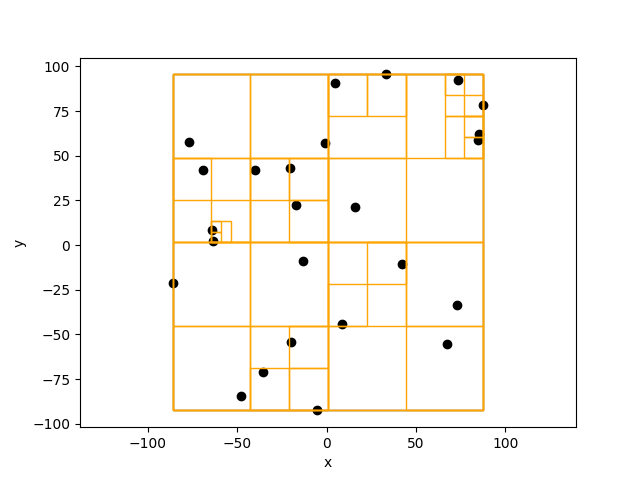
\includegraphics[width=7.9cm]{obrazy/png/random_uniform_test_quad.png} }}%
    \qquad
    \subfloat[\centering Rozkład jednostajny - KdTree]{{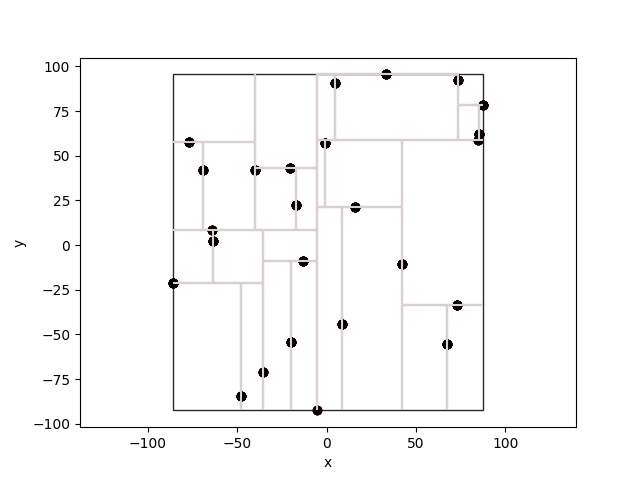
\includegraphics[width=7.9cm]{obrazy/png/random_uniform_test_kd.png} }}%
    \caption{Struktury po inicjalizacji dla rozkładu jednostajnego}%
    \label{fig:random_uniform}%
\end{figure}

\begin{figure}[h]
    \centering
    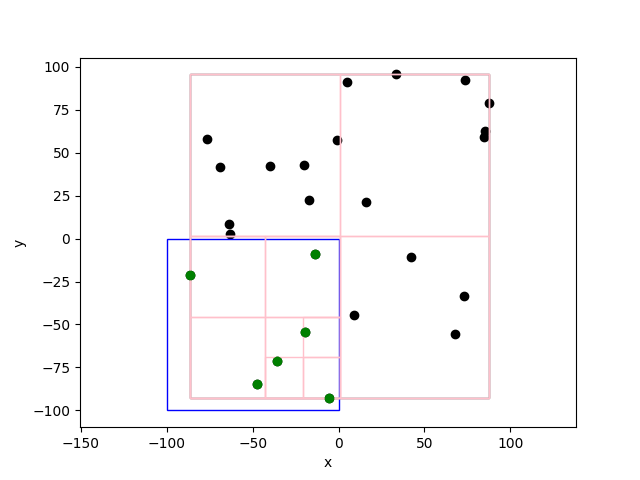
\includegraphics[width=0.6\linewidth]{obrazy/png/random_uniform_test_quad_result.png}
    \caption{Wykres przedstawiający wynik testu "rozkład jednostajny" dla \texttt{QuadTree}}
    \label{fig:random_uniform_test_quad_result}
\end{figure}

\nopagebreak
\begin{table}[h]
\centering
\caption{Wyniki dla rozkładu jednostajnego}
\label{tab:random_uniform_test}
\begin{tabular}{ccccc}
\toprule
\multirow{2}{*}{\textbf{Rozmiar}} & \multicolumn{2}{c}{\textbf{Czas budowy [s]}} & \multicolumn{2}{c}{\textbf{Czas zapytania [s]}} \\
\cmidrule(lr){2-3} \cmidrule(lr){4-5}
 & \textbf{KD} & \textbf{Quad} & \textbf{KD} & \textbf{Quad} \\
\midrule
1000   & 0.018922 & 0.058033 & 0.000010 & 0.000015 \\
5000   & 0.095042 & 0.269483 & 0.000035 & 0.000042 \\
10000  & 0.171406 & 0.529662 & 0.000057 & 0.000062 \\
20000  & 0.366894 & 1.106446 & 0.000073 & 0.000089 \\
40000  & 0.738852 & 2.073481 & 0.000113 & 0.000151 \\
60000  & 1.087992 & 3.158903 & 0.000172 & 0.000230 \\
80000  & 1.448442 & 4.463680 & 0.000223 & 0.000289 \\
100000 & 1.803712 & 5.683522 & 0.000277 & 0.000343 \\
\bottomrule
\end{tabular}
\end{table}

\nopagebreak
\begin{figure}[h]
    \centering
    \includegraphics[width=1\linewidth]{obrazy/tests/random_uniform_test.png}
    \caption{Wykres porównujący wydajność QuadTree i KdTree dla rozkładu jednostajnego}
    \label{fig:random_uniform_tests}
\end{figure}

\noindent Na podstawie wyników zawartych w tabeli (\ref{tab:random_uniform_test}) oraz wykresu (\ref{fig:random_uniform_tests}) można zauważyć, że dla danych generowanych równomiernie w przestrzeni dwuwymiarowej, struktura \texttt{KdTree} charakteryzuje się wyraźnie krótszym czasem budowy w porównaniu do \texttt{QuadTree}. Średni czas budowy \texttt{KdTree} jest o około 60\% krótszy niż dla \texttt{QuadTree}. 

\noindent Dla zapytań struktura \texttt{KdTree} osiąga minimalnie lepsze wyniki, co wynika z efektywnego podziału przestrzeni i mniejszej liczby przeszukiwanych węzłów. Na wykresie (\ref{fig:random_uniform_tests}), którego skala osi OX jest logarytmiczna, widać, że \texttt{KdTree} ma w przypadku zapytań przewagę czasową nad \texttt{QuadTree}, choć różnica jest niewielka.

\pagebreak

\subsection{Rozkład normalny}
Modelowanie skupionych danych pozwala na analizę, jak struktury działają, gdy punkty są skoncentrowane wokół jednego miejsca. Punkty są generowane zgodnie z rozkładem normalnym.
\begin{itemize}
    \item \textbf{Opis}: Punkty generowane zgodnie z rozkładem normalnym o zadanej średniej \( \mu \) i odchyleniu standardowym \( \sigma \).
    \item \textbf{Prostokąt przeszukiwania}: Zawiera dolną lewą ćwiartkę przestrzeni wokół średniej rozkładu.
    \item \textbf{Zastosowanie}: Modelowanie skupionych danych, które występują częściej w określonych miejscach przestrzeni.
\end{itemize}

\begin{figure}[h]
    \centering
    \subfloat[\centering Rozkład normalny - QuadTree]{{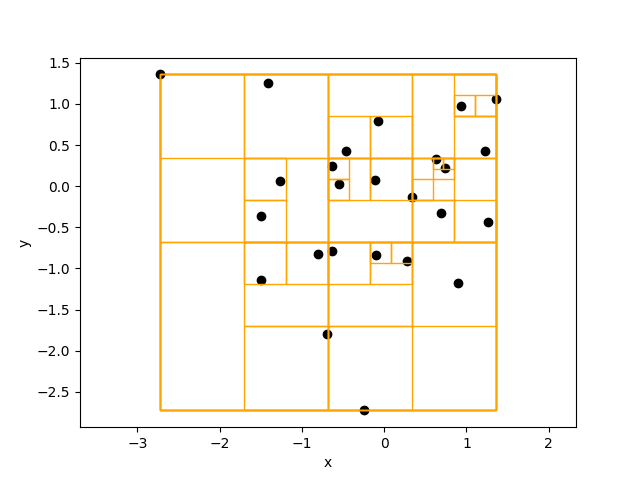
\includegraphics[width=7.9cm]{obrazy/png/random_normal_test_quad.png} }}%
    \qquad
    \subfloat[\centering Rozkład normalny - KdTree]{{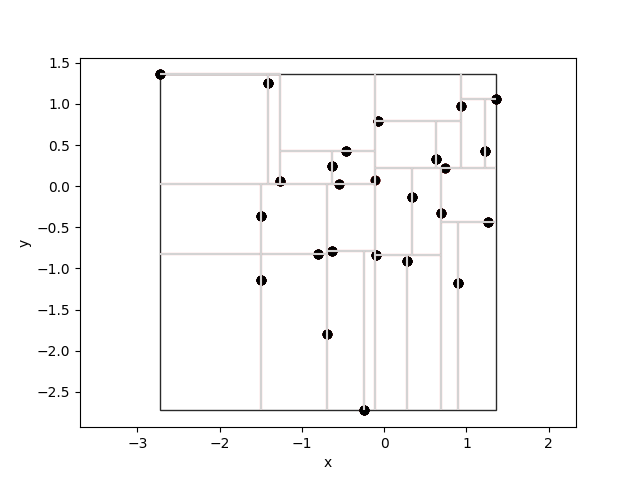
\includegraphics[width=7.9cm]{obrazy/png/random_normal_test_kd.png} }}%
    \caption{Struktury po inicjalizacji dla rozkładu normalnego punktów}%
    \label{fig:random_normal}%
\end{figure}

\begin{figure}[h]
    \centering
    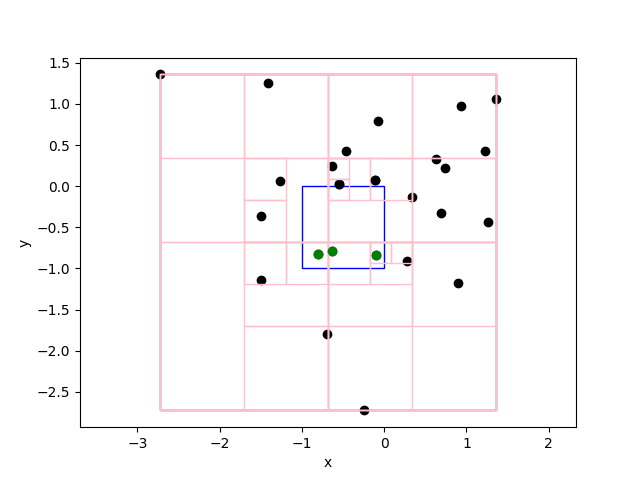
\includegraphics[width=0.6\linewidth]{obrazy/png/random_normal_test_quad_result.png}
    \caption{Wykres przedstawiający wynik testu "Rozkład normalny" dla \texttt{QuadTree}}
    \label{fig:random_normal_test_quad_result}
\end{figure}

\begin{table}[h]
\centering
\caption{Wyniki dla rozkładu normalnego punktów}
\label{tab:random_normal_test}
\begin{tabular}{ccccc}
\toprule
\multirow{2}{*}{\textbf{Rozmiar}} & \multicolumn{2}{c}{\textbf{Czas budowy [s]}} & \multicolumn{2}{c}{\textbf{Czas zapytania [s]}} \\
\cmidrule(lr){2-3} \cmidrule(lr){4-5}
 & \textbf{KD} & \textbf{Quad} & \textbf{KD} & \textbf{Quad} \\
\midrule
1000   & 0.019210 & 0.057586 & 0.000525 & 0.000845 \\
5000   & 0.095701 & 0.269673 & 0.002444 & 0.003690 \\
10000  & 0.172891 & 0.559579 & 0.004762 & 0.007883 \\
20000  & 0.369092 & 1.088995 & 0.009385 & 0.013987 \\
40000  & 0.743298 & 2.179939 & 0.018621 & 0.029733 \\
60000  & 1.095386 & 3.356612 & 0.028484 & 0.045621 \\
80000  & 1.449910 & 4.381948 & 0.038525 & 0.060902 \\
100000 & 1.805228 & 5.497975 & 0.048460 & 0.076501 \\
\bottomrule
\end{tabular}
\end{table}

\begin{figure}[h]
    \centering
    \includegraphics[width=1\linewidth]{obrazy/tests/random_normal_test.png}
    \caption{Wykres porównujący wydajność QuadTree i KdTree dla rozkładu normalnego punktów.}
    \label{fig:random_normal_tests}
\end{figure}


\newpage
\noindent Analiza wyników z tabeli (\ref{tab:random_normal_test}) oraz wykresu (\ref{fig:random_normal_tests}) wskazuje, że \texttt{KdTree} dominuje nad \texttt{QuadTree} zarówno pod względem czasu budowy, jak i zapytań dla danych o rozkładzie normalnym. Średni czas budowy \texttt{KdTree} jest o około 60\% krótszy, co świadczy o dobrej wydajności tej struktury w przypadku danych bardziej skupionych w centrum przestrzeni.

\noindent W przypadku zapytań różnica czasów jest niewielka, co sugeruje, że złożoność obu struktur przy danych skoncentrowanych wokół środka jest podobna. Niemniej jednak, czas budowy wyraźnie wskazuje na przewagę \texttt{KdTree} w takich warunkach.

\newpage
\subsection{Współrzędne całkowite}
Test danych dyskretnych ma na celu ocenę zdolności struktur do pracy z danymi, które nie są rozłożone równomiernie w przestrzeni ciągłej. Dodatkowo pozwala sprawdzić poprawność zliczania duplikatów.
\begin{itemize}
    \item \textbf{Opis}: Zbiór punktów losowo generowanych jako liczby całkowite w zadanym przedziale \texttt{[minval, maxval]}.
    \item \textbf{Prostokąt przeszukiwania}: Zawiera dolną lewą ćwiartkę przestrzeni.
    \item \textbf{Zastosowanie}: Testowanie struktur na danych dyskretnych.
\end{itemize}

\begin{figure}[h]
    \centering
    \subfloat[\centering Współrzędne całkowite - QuadTree]{{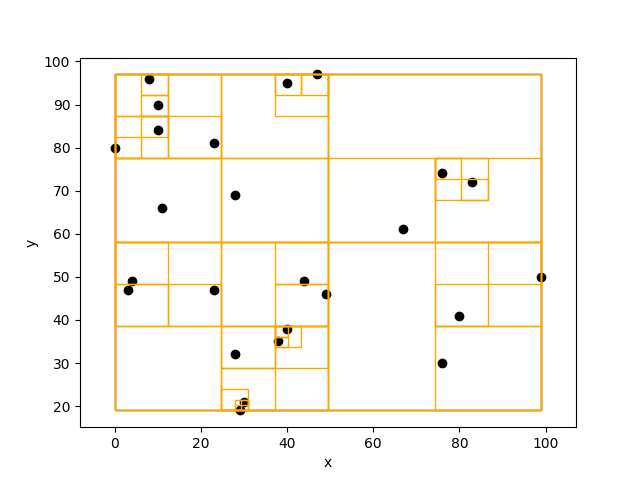
\includegraphics[width=7.9cm]{obrazy/png/random_integer_test_quad.png} }}%
    \qquad
    \subfloat[\centering Współrzędne całkowite - KdTree]{{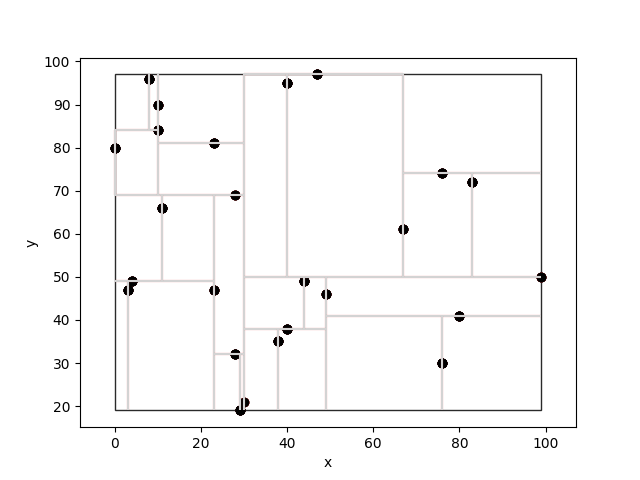
\includegraphics[width=7.9cm]{obrazy/png/random_integer_test_kd.png} }}%
    \caption{Struktury po inicjalizacji dla testu "Współrzędne całkowite"}%
    \label{fig:random_integer}%
\end{figure}

\begin{figure}[h]
    \centering
    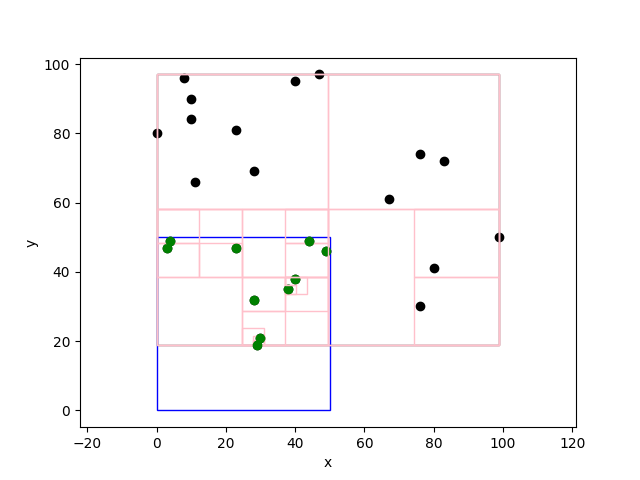
\includegraphics[width=0.6\linewidth]{obrazy/png/random_integer_test_quad_result.png}
    \caption{Wykres przedstawiający wynik testu "Współrzędne całkowite" dla \texttt{QuadTree}}
    \label{fig:random_integer_test_quad_result}
\end{figure}

\begin{table}[h]
\centering
\caption{Wyniki dla testu "Współrzędne całkowite"}
\label{tab:random_integer_test}
\begin{tabular}{ccccc}
\toprule
\multirow{2}{*}{\textbf{Rozmiar}} & \multicolumn{2}{c}{\textbf{Czas budowy [s]}} & \multicolumn{2}{c}{\textbf{Czas zapytania [s]}} \\
\cmidrule(lr){2-3} \cmidrule(lr){4-5}
 & \textbf{KD} & \textbf{Quad} & \textbf{KD} & \textbf{Quad} \\
\midrule
1000   & 0.019829 & 0.058950 & 0.005241 & 0.006265 \\
5000   & 0.094284 & 0.274114 & 0.021957 & 0.028869 \\
10000  & 0.191404 & 0.538868 & 0.043555 & 0.050724 \\
20000  & 0.362148 & 1.092364 & 0.083759 & 0.099803 \\
40000  & 0.706396 & 2.012272 & 0.161121 & 0.187673 \\
60000  & 1.009903 & 2.907660 & 0.229637 & 0.268951 \\
80000  & 1.291108 & 3.951865 & 0.297839 & 0.356040 \\
100000 & 1.557419 & 4.967314 & 0.359130 & 0.433662 \\
\bottomrule
\end{tabular}
\end{table}

\begin{figure}[h]
    \centering
    \includegraphics[width=1\linewidth]{obrazy/tests/random_integer_test.png}
    \caption{Wykres porównujący wydajność QuadTree i KdTree dla testu "Współrzędne całkowite"}
    \label{fig:random_integer_tests}
\end{figure}

\newpage
\noindent Z danych w tabeli (\ref{tab:random_integer_test}) oraz wykresu (\ref{fig:random_integer_tests}) wynika, że \texttt{KdTree} jest bardziej wydajna zarówno w budowie, jak i przeszukiwaniu dla danych dyskretnych. Średni czas budowy \texttt{KdTree} jest o około 65\% krótszy niż dla \texttt{QuadTree}, co pokazuje jej efektywność w obsłudze punktów o wartościach całkowitych.

\noindent Analiza wyników testu dla danych typu integer pokazuje, że \texttt{QuadTree} osiąga lepsze wyniki w czasie zapytań w porównaniu do \texttt{KdTree}.

\noindent Ten test, obejmujący dane o dyskretnych wartościach, dodatkowo bardzo skutecznie sprawdza poprawność zliczania duplikatów. Poprawne zliczanie takich punktów umożliwia dokładną analizę danych oraz zapewnia, że struktury są w stanie poprawnie przechowywać i obsługiwać wielokrotne wystąpienia tego samego punktu w przestrzeni.

\noindent Struktura \texttt{KdTree}, bazująca na wyborze mediany podczas podziału, może w niektórych przypadkach wykazywać trudności w równomiernym przetwarzaniu dużej liczby duplikatów, szczególnie gdy są one skoncentrowane w jednym wymiarze. Natomiast \texttt{QuadTree}, dzięki podziałowi przestrzeni na mniejsze obszary bez względu na wartości punktów, lepiej radzi sobie z danymi tego rodzaju, co czyni ją bardziej stabilną i niezawodną przy obsłudze dyskretnych wartości.


\newpage
\subsection{Siatka}
Dane o regularnym rozmieszczeniu, takie jak siatki, są częste w grafice komputerowej i analizie przestrzennej. Test ten ocenia, jak struktury radzą sobie z powtarzalnymi wzorcami w danych.
\begin{itemize}
    \item \textbf{Opis}: Punkty rozmieszczone równomiernie na siatce w przestrzeni dwuwymiarowej \texttt{[minval, maxval]}.
    \item \textbf{Prostokąt przeszukiwania}: Zawiera dolną lewą ćwiartkę siatki.
    \item \textbf{Zastosowanie}: Modelowanie danych przestrzennych o regularnym rozmieszczeniu.
\end{itemize}

\begin{figure}[h]
    \centering
    \subfloat[\centering Siatka - QuadTree]{{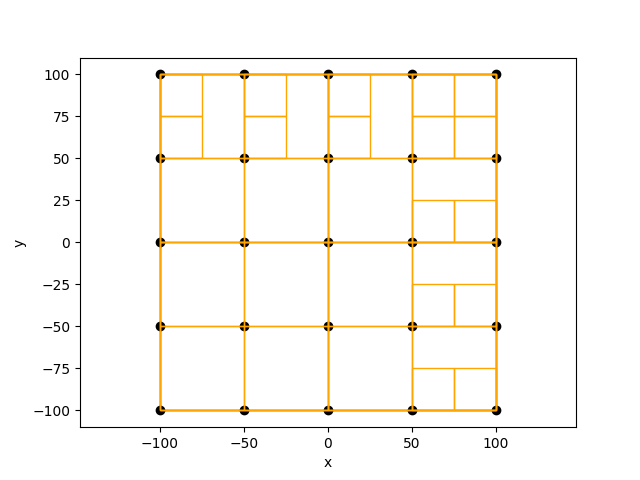
\includegraphics[width=7.9cm]{obrazy/png/grid_test_quad.png} }}%
    \qquad
    \subfloat[\centering Siatka - KdTree]{{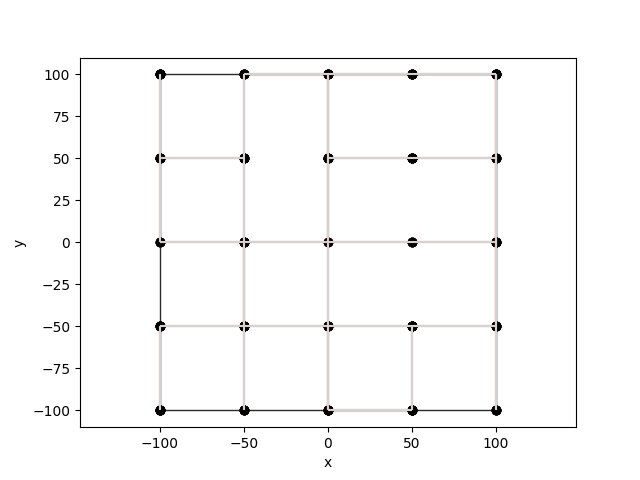
\includegraphics[width=7.9cm]{obrazy/png/grid_test_kd.png} }}%
    \caption{Struktury po inicjalizacji dla testu "Siatka"}%
    \label{fig:grid}%
\end{figure}
\begin{figure}[h]
    \centering
    \includegraphics[width=0.6\linewidth]{obrazy/png/to_rename.png}
    \caption{Wykres przedstawiający wynik testu "Siatka" dla \texttt{QuadTree}}
    \label{fig:grid_test_quad_result}
\end{figure}
\begin{table}[h]
\centering
\caption{Wyniki dla testu "Siatka"}
\label{tab:grid_test}
\begin{tabular}{cccccc}
\toprule
\multirow{2}{*}{\textbf{Rozmiar}} & \multicolumn{2}{c}{\textbf{Czas budowy [s]}} & \multicolumn{2}{c}{\textbf{Czas zapytania [s]}} \\
\cmidrule(lr){2-3} \cmidrule(lr){4-5}
 & \textbf{KD} & \textbf{Quad} & \textbf{KD} & \textbf{Quad} \\
\midrule
1000   & 0.016031 & 0.027798 & 0.000217 & 0.000248 \\
5000   & 0.082159 & 0.220597 & 0.001088 & 0.001352 \\
10000  & 0.167333 & 0.440548 & 0.002262 & 0.002847 \\
20000  & 0.335196 & 0.926937 & 0.004406 & 0.006215 \\
40000  & 0.677760 & 1.787519 & 0.009231 & 0.011793 \\
60000  & 1.002867 & 1.846243 & 0.013598 & 0.015832 \\
80000  & 1.356284 & 3.950726 & 0.017787 & 0.027986 \\
100000 & 1.742447 & 5.603694 & 0.022990 & 0.036359 \\
\bottomrule
\end{tabular}
\end{table}
\begin{figure}[h]
    \centering
    \includegraphics[width=1\linewidth]{obrazy/tests/grid_test.png}
    \caption{Wykres porównujący wydajność QuadTree i KdTree dla testu "Siatka"}
    \label{fig:grid_tests}
\end{figure}
\newpage
\noindent Na podstawie tabeli (\ref{tab:grid_test}) oraz wykresu (\ref{fig:grid_tests}) można zauważyć, że w przypadku danych rozmieszczonych na siatce, \texttt{KdTree} jest zdecydowanie szybsza w budowie, z czasem budowy krótszym średnio o 64\% w porównaniu do \texttt{QuadTree}. 

\noindent Czas zapytań dla obu struktur jest bardzo zbliżony, co sugeruje, że zarówno \texttt{KdTree}, jak i \texttt{QuadTree} są odpowiednie do obsługi danych o regularnym rozmieszczeniu, choć czas budowy wskazuje na wyraźną przewagę \texttt{KdTree}.



\newpage

\subsection{Okrąg}
Rozmieszczenie punktów na okręgu pozwala zbadać, jak struktury radzą sobie z danymi o specyficznej geometrii, które nie są równomierne ani skupione.
\begin{itemize}
    \item \textbf{Opis}: Punkty rozmieszczone równomiernie na okręgu o zadanym promieniu.
    \item \textbf{Prostokąt przeszukiwania}: Zawiera centralny fragment okręgu.
    \item \textbf{Zastosowanie}: Testowanie struktur dla danych o specyficznej geometrii.
\end{itemize}

\begin{figure}[h]
    \centering
    \subfloat[\centering Okrąg - QuadTree]{{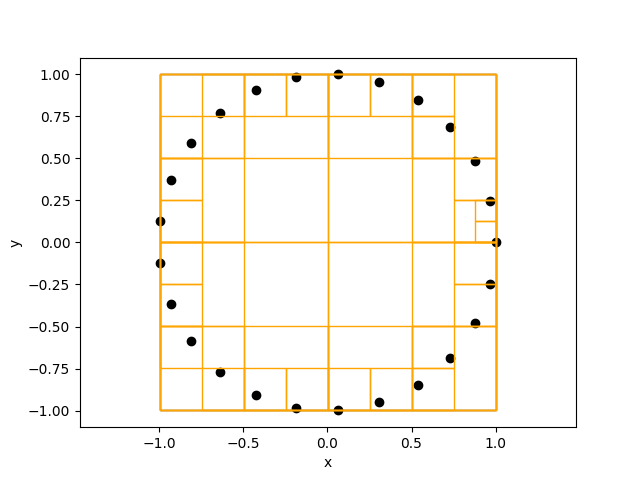
\includegraphics[width=7.9cm]{obrazy/png/circle_test_quad.png} }}%
    \qquad
    \subfloat[\centering Okrąg - KdTree]{{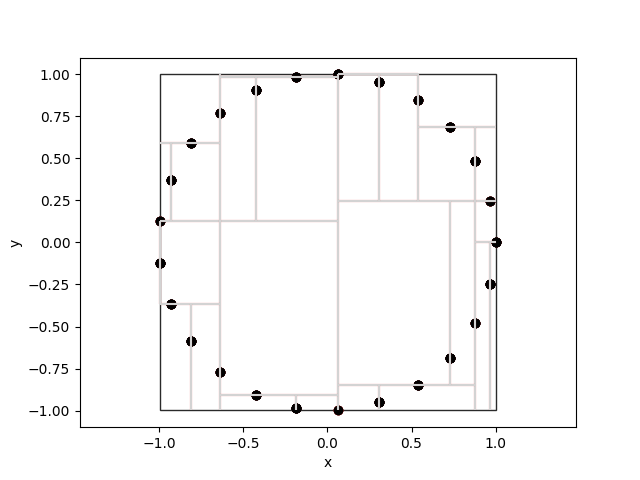
\includegraphics[width=7.9cm]{obrazy/png/circle_test_kd.png} }}%
    \caption{Struktury po inicjalizacji dla testu "Okrąg"}%
    \label{fig:circle}%
\end{figure}
\begin{figure}[h]
    \centering
    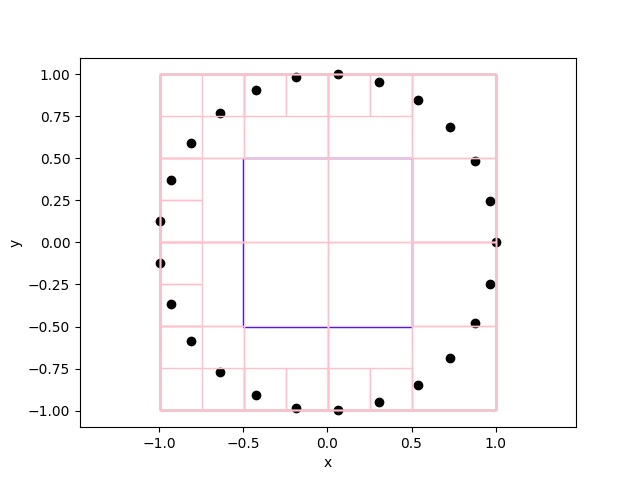
\includegraphics[width=0.6\linewidth]{obrazy/png/circle_test_quad_result.png}
    \caption{Wykres przedstawiający wynik testu "Okrąg" dla \texttt{QuadTree}}
    \label{fig:circle_test_quad_result}
\end{figure}
\begin{table}[h]
\centering
\caption{Wyniki dla testu "Okrąg"}
\label{tab:circle_test}
\begin{tabular}{ccccc}
\toprule
\multirow{2}{*}{\textbf{Rozmiar}} & \multicolumn{2}{c}{\textbf{Czas budowy [s]}} & \multicolumn{2}{c}{\textbf{Czas zapytania [s]}} \\
\cmidrule(lr){2-3} \cmidrule(lr){4-5}
 & \textbf{KD} & \textbf{Quad} & \textbf{KD} & \textbf{Quad} \\
\midrule
1000   & 0.017224 & 0.049405 & 0.000283 & 0.000384 \\
5000   & 0.085444 & 0.342690 & 0.001402 & 0.002219 \\
10000  & 0.171450 & 0.691201 & 0.002798 & 0.004350 \\
20000  & 0.346181 & 1.397290 & 0.005673 & 0.008968 \\
40000  & 0.705842 & 2.817965 & 0.011353 & 0.018113 \\
60000  & 1.056654 & 4.036513 & 0.017351 & 0.029915 \\
80000  & 1.418979 & 5.572406 & 0.023283 & 0.039219 \\
100000 & 1.769146 & 5.764479 & 0.029173 & 0.047566 \\
\bottomrule
\end{tabular}
\end{table}

\begin{figure}[h]
    \centering
    \includegraphics[width=1\linewidth]{obrazy/tests/circle_test.png}
    \caption{Wykres porównujący wydajność QuadTree i KdTree dla testu "Okrąg"}
    \label{fig:circle_tests}
\end{figure}

\newpage
\noindent Dane w tabeli (\ref{tab:circle_test}) oraz wykres (\ref{fig:circle_tests}) wskazują, że \texttt{KdTree} jest znacznie szybsza w budowie w przypadku danych rozmieszczonych na okręgu, osiągając średni czas budowy krótszy o około 70\%. Wynika to z efektywnego podziału przestrzeni przez tę strukturę.

\noindent W przypadku zapytań wyraźną przewagę zyskuje \texttt{QuadTree}, która dzięki mechanizmowi sprawdzania przecięć prostokątów odwiedza jedynie istotne węzły. Skala logarytmiczna wykresu pokazuje, że czas zapytań dla \texttt{QuadTree} jest krótszy niż dla \texttt{KdTree}. Dzięki temu \texttt{QuadTree} może być szczególnie przydatna w aplikacjach wymagających licznych operacji przeszukiwania na danych o skomplikowanej geometrii.


\newpage
\subsection{Prosta}
Współliniowe dane to wyzwanie dla struktur danych, które bazują na podziale przestrzeni. Test ten pozwala zbadać, czy struktury są w stanie efektywnie obsłużyć takie sytuacje.
\begin{itemize}
    \item \textbf{Opis}: Punkty rozmieszczone równomiernie na linii łączącej dwa zdefiniowane punkty \( (x_1, y_1) \) i \( (x_2, y_2) \).
    \item \textbf{Prostokąt przeszukiwania}: Fragment linii w dolnej lewej ćwiartce.
    \item \textbf{Zastosowanie}: Analiza wydajności przy współliniowych danych.
\end{itemize}

\begin{figure}[h]
    \centering
    \subfloat[\centering Prosta - QuadTree]{{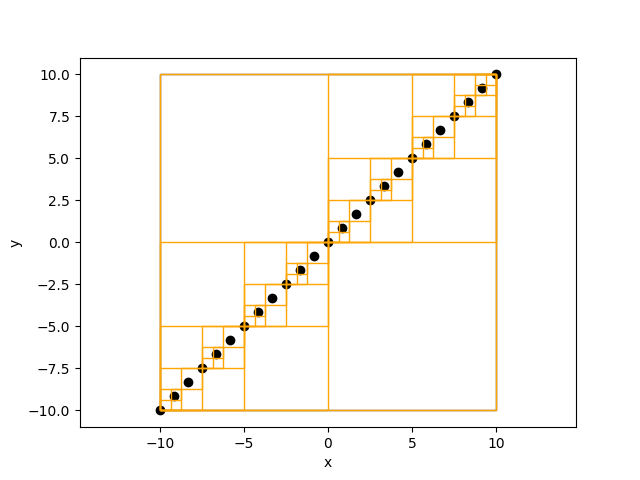
\includegraphics[width=7.9cm]{obrazy/png/line_test_quad.png} }}%
    \qquad
    \subfloat[\centering Prosta - KdTree]{{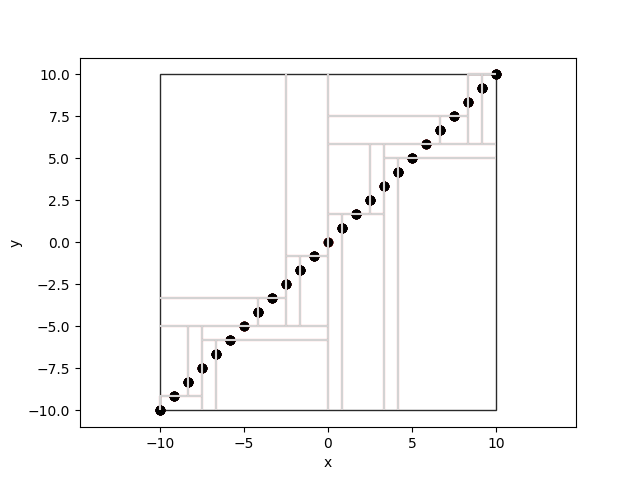
\includegraphics[width=7.9cm]{obrazy/png/line_test_kd.png} }}%
    \caption{Struktury po inicjalizacji dla testu "Prosta"}%
    \label{fig:line}%
\end{figure}

\begin{figure}[h]
    \centering
    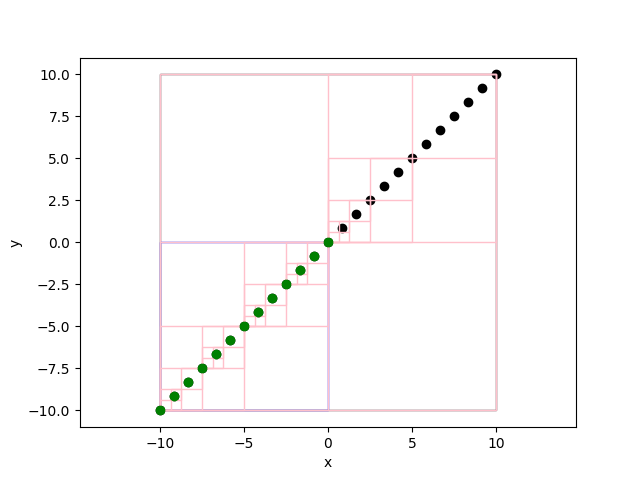
\includegraphics[width=0.6\linewidth]{obrazy/png/line_test_quad_result.png}
    \caption{Wykres przedstawiający wynik testu "Prosta" dla \texttt{QuadTree}}
    \label{fig:line_test_quad_result}
\end{figure}

\begin{table}[h]
\centering
\caption{Wyniki dla testu "Prosta"}
\label{tab:line_test}
\begin{tabular}{ccccc}
\toprule
\multirow{2}{*}{\textbf{Rozmiar}} & \multicolumn{2}{c}{\textbf{Czas budowy [s]}} & \multicolumn{2}{c}{\textbf{Czas zapytania [s]}} \\
\cmidrule(lr){2-3} \cmidrule(lr){4-5}
 & \textbf{KD} & \textbf{Quad} & \textbf{KD} & \textbf{Quad} \\
\midrule
1000   & 0.018888 & 0.042949 & 0.000594 & 0.000880 \\
5000   & 0.087099 & 0.325811 & 0.003363 & 0.006222 \\
10000  & 0.192269 & 0.672375 & 0.006005 & 0.009878 \\
20000  & 0.369080 & 1.326105 & 0.012120 & 0.020459 \\
40000  & 0.745303 & 2.661519 & 0.024606 & 0.044176 \\
60000  & 1.097186 & 2.930981 & 0.037441 & 0.059906 \\
80000  & 1.454449 & 5.381592 & 0.050701 & 0.090368 \\
100000 & 1.815930 & 5.814215 & 0.065322 & 0.107913 \\
\bottomrule
\end{tabular}
\end{table}

\begin{figure}[h]
    \centering
    \includegraphics[width=1\linewidth]{obrazy/tests/line_test.png}
    \caption{Wykres porównujący wydajność QuadTree i KdTree dla testu "Prosta"}
    \label{fig:line_tests}
\end{figure}

\newpage
\noindent Analiza tabeli (\ref{tab:line_test}) oraz wykresu (\ref{fig:line_tests}) pokazuje, że w przypadku danych współliniowych, \texttt{KdTree} osiąga lepsze wyniki zarówno w czasie budowy, jak i zapytań. W teście "Prosta" punkty są rozmieszczone równomiernie na linii prostej, co sprawia, że charakterystyka danych jest wyjątkowo regularna i łatwa do obsługi dla struktur opartych na podziałach przestrzeni.

\noindent Z kolei \texttt{QuadTree}, pomimo swojej zdolności do precyzyjnego podziału przestrzeni na mniejsze regiony, w przypadku danych współliniowych tworzy wiele zbędnych podziałów, które nie prowadzą do optymalizacji. W efekcie liczba węzłów przeszukiwanych w tej strukturze jest większa, co wydłuża czas zapytań.

\newpage
\subsection{Krzyż}
Rozmieszczenie punktów wzdłuż dwóch przecinających się linii, prostopadłych do osi układu współrzędnych, pozwala ocenić efektywność struktur w sytuacjach, gdy dane są liniowo rozmieszczone w więcej niż jednym kierunku.
\begin{itemize}
    \item \textbf{Opis}: Punkty rozmieszczone wzdłuż osi \( x = 0 \) oraz \( y = 0 \), tworząc krzyż w przestrzeni dwuwymiarowej.
    \item \textbf{Prostokąt przeszukiwania}: Centralny fragment osi.
    \item \textbf{Zastosowanie}: Testowanie efektywności struktur przy danych rozmieszczonych liniowo w dwóch wymiarach.
\end{itemize}

\begin{figure}[h]
    \centering
    \subfloat[\centering Krzyż - QuadTree]{{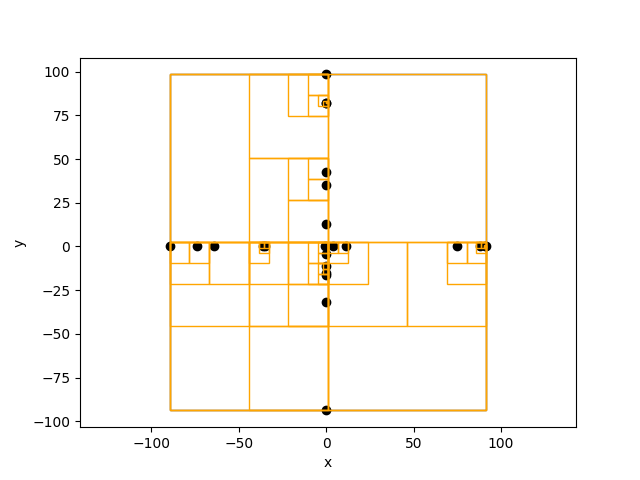
\includegraphics[width=7.9cm]{obrazy/png/cross_test_quad.png} }}%
    \qquad
    \subfloat[\centering Krzyż - KdTree]{{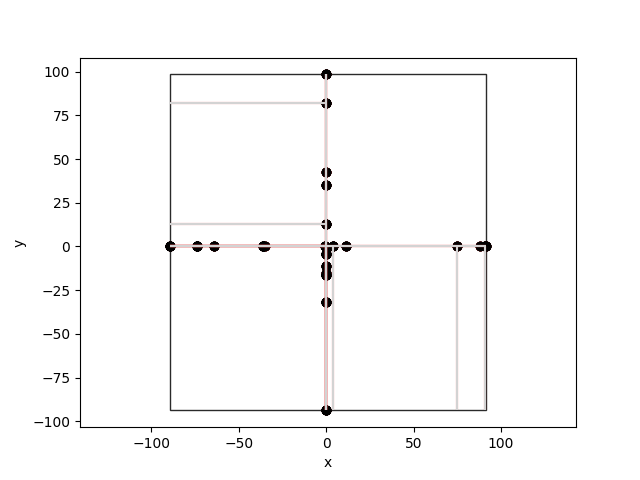
\includegraphics[width=7.9cm]{obrazy/png/cross_test_kd.png} }}%
    \caption{Struktury po inicjalizacji dla testu "Krzyż"}%
    \label{fig:cross}%
\end{figure}

\begin{figure}[h]
    \centering
    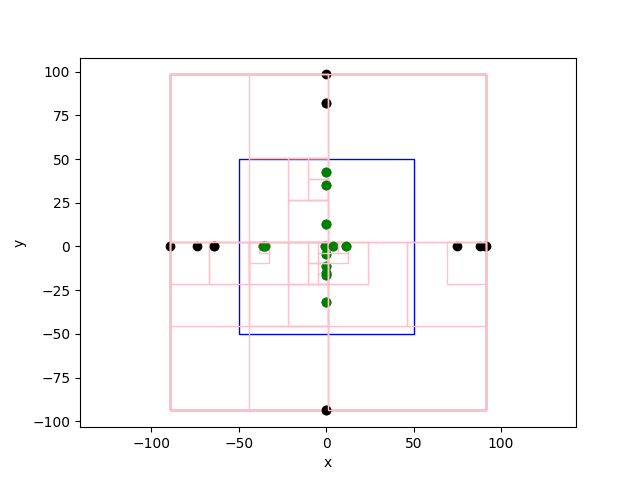
\includegraphics[width=0.6\linewidth]{obrazy/png/cross_test_quad_result.png}
    \caption{Wykres przedstawiający wynik testu "Krzyż" dla \texttt{QuadTree}}
    \label{fig:cross_test_quad_result}
\end{figure}

\begin{table}[h]
\centering
\caption{Wyniki dla testu "Krzyż"}
\label{tab:cross_test}
\begin{tabular}{cccccc}
\toprule
\multirow{2}{*}{\textbf{Rozmiar}} & \multicolumn{2}{c}{\textbf{Czas budowy [s]}} & \multicolumn{2}{c}{\textbf{Czas zapytania [s]}} \\
\cmidrule(lr){2-3} \cmidrule(lr){4-5}
 & \textbf{KD} & \textbf{Quad} & \textbf{KD} & \textbf{Quad} \\
\midrule
1000   & 0.018981 & 0.064886 & 0.000507 & 0.000693 \\
5000   & 0.095953 & 0.304825 & 0.002354 & 0.003687 \\
10000  & 0.194218 & 0.635394 & 0.004606 & 0.006449 \\
20000  & 0.374248 & 1.263960 & 0.009680 & 0.013568 \\
40000  & 0.755895 & 2.541623 & 0.019337 & 0.028854 \\
60000  & 1.120899 & 3.849832 & 0.029624 & 0.043147 \\
80000  & 1.480665 & 5.155926 & 0.039191 & 0.058023 \\
100000 & 1.828316 & 6.582835 & 0.049956 & 0.072920 \\
\bottomrule
\end{tabular}
\end{table}

\begin{figure}[h]
    \centering
    \includegraphics[width=1\linewidth]{obrazy/tests/cross_test.png}
    \caption{Wykres porównujący wydajność QuadTree i KdTree dla testu "Krzyż"}
    \label{fig:cross_tests}
\end{figure}

\newpage
\noindent Wyniki z tabeli (\ref{tab:cross_test}) oraz wykresu (\ref{fig:cross_tests}) wskazują na  przewagę \texttt{KdTree} w przypadku danych rozmieszczonych wzdłuż osi układu współrzędnych. Czas budowy \texttt{KdTree} jest krótszy o około 40\%, co wynika z jej efektywnego podejścia do podziału przestrzeni, które lepiej radzi sobie z liniowym rozmieszczeniem danych w jednym wymiarze.

\noindent Dla zapytań \texttt{KdTree} również osiąga lepsze wyniki, z czasem zapytań krótszym o około 35\%. Efektywność \texttt{KdTree} w tym przypadku wynika z jej struktury hierarchicznej, która pozwala szybciej ograniczyć liczbę przeszukiwanych punktów dzięki podziałom przestrzeni wzdłuż osi.


\newpage
\subsection{Boki prostokąta}
Rozmieszczenie punktów wzdłuż boków prostokąta symuluje dane, które znajdują się na granicach przestrzeni.
\begin{itemize}
    \item \textbf{Opis}: Punkty rozmieszczone wzdłuż boków prostokąta w przestrzeni dwuwymiarowej.
    \item \textbf{Prostokąt przeszukiwania}: Fragment zawierający dolną lewą ćwiartkę prostokąta.
    \item \textbf{Zastosowanie}: Analiza wydajności struktur dla danych znajdujących się na krawędziach.
\end{itemize}

\begin{figure}[h]
    \centering
    \subfloat[\centering Boki prostokąta - QuadTree]{{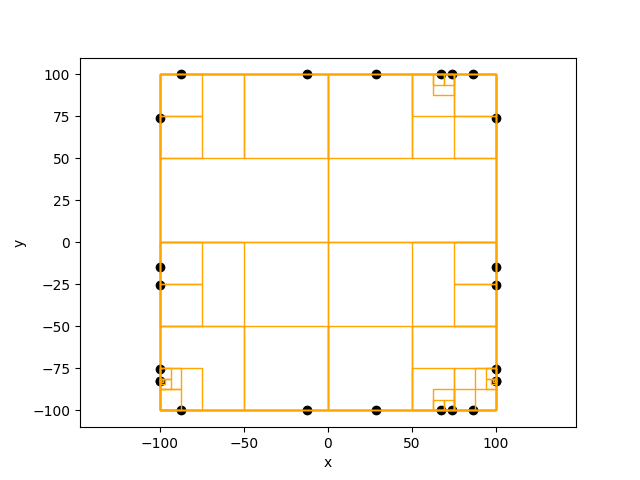
\includegraphics[width=7.9cm]{obrazy/png/rectangle_sides_test_quad.png} }}%
    \qquad
    \subfloat[\centering Boki prostokąta - KdTree]{{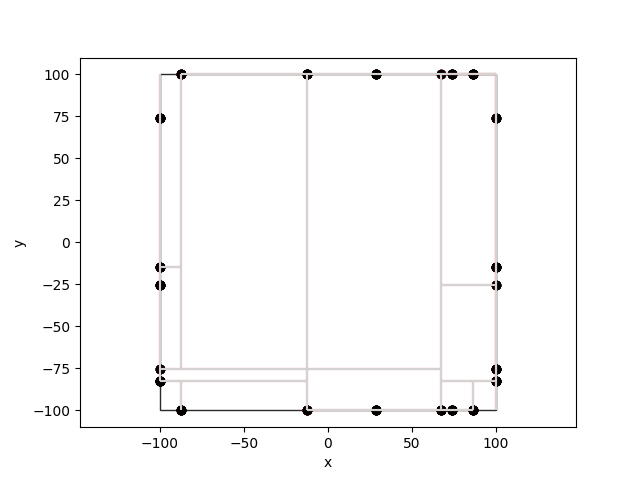
\includegraphics[width=7.9cm]{obrazy/png/rectangle_sides_test_kd.png} }}%
    \caption{Struktury po inicjalizacji dla testu "Boki prostokąta"}%
    \label{fig:rectangle_sides}%
\end{figure}

\begin{figure}[h]
    \centering
    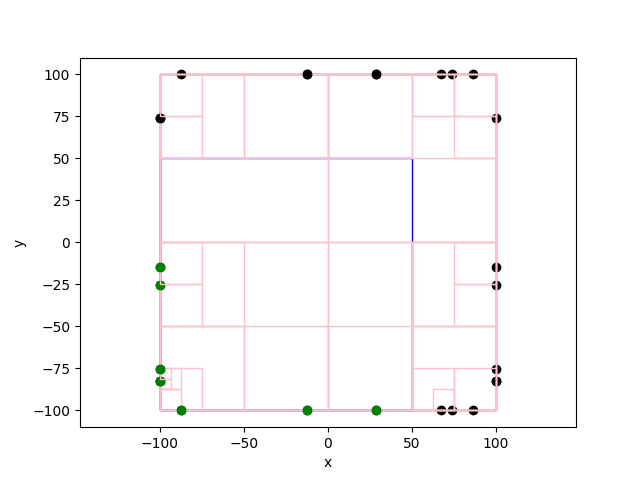
\includegraphics[width=0.6\linewidth]{obrazy/png/rectangle_sides_test_quad_result.png}
    \caption{Wykres przedstawiający wynik testu "Boki prostokąta" dla \texttt{QuadTree}}
    \label{fig:rectangle_sides_test_quad_result}
\end{figure}

\begin{table}[h]
\centering
\caption{Wyniki dla testu "Boki prostokąta"}
\label{tab:rectangle_sides}
\begin{tabular}{cccccc}
\toprule
\multirow{2}{*}{\textbf{Rozmiar}} & \multicolumn{2}{c}{\textbf{Czas budowy [s]}} & \multicolumn{2}{c}{\textbf{Czas zapytania [s]}} \\
\cmidrule(lr){2-3} \cmidrule(lr){4-5}
 & \textbf{KD} & \textbf{Quad} & \textbf{KD} & \textbf{Quad} \\
\midrule
1000   & 0.020787 & 0.059019 & 0.000642 & 0.000500 \\
5000   & 0.124461 & 0.291517 & 0.002962 & 0.002344 \\
10000  & 0.350367 & 0.602067 & 0.006162 & 0.004796 \\
20000  & 1.001281 & 1.278985 & 0.014031 & 0.012119 \\
40000  & 2.995309 & 2.466272 & 0.024968 & 0.021562 \\
60000  & 6.078603 & 3.762051 & 0.039082 & 0.034486 \\
80000  & 10.623845 & 5.082895 & 0.052354 & 0.046869 \\
100000 & 37.890306 & 6.314411 & 0.065584 & 0.060417 \\
\bottomrule
\end{tabular}
\end{table}
\begin{figure}[h]
    \centering
    \includegraphics[width=1\linewidth]{obrazy/tests/rectangle_sides_test.png}
    \caption{Wykres porównujący wydajność QuadTree i KdTree dla testu "Boki prostokąta"}
    \label{fig:rectangle_sides_tests}
\end{figure}

\newpage
\noindent Wyniki przedstawione w tabeli (\ref{tab:rectangle_sides}) oraz na wykresie (\ref{fig:rectangle_sides_tests}) wskazują, że w przypadku danych rozmieszczonych wzdłuż boków prostokąta \texttt{QuadTree} początkowo osiąga wyniki zbliżone do \texttt{KdTree}, jednak wraz ze wzrostem liczby punktów zaczyna wykazywać coraz większą przewagę.

\noindent Dla większych zbiorów danych czas budowy \texttt{QuadTree} jest krótszy o około 48\%, co wynika z precyzyjnego podziału przestrzeni na mniejsze obszary, dostosowanych do danych znajdujących się na granicach prostokąta. Czas zapytań \texttt{QuadTree} jest krótszy o około 55\%, co potwierdza efektywność tej struktury w sytuacjach, gdzie punkty znajdują się głównie na krawędziach przestrzeni.

\noindent Na wykresach w skali logarytmicznej (rysunek \ref{fig:rectangle_sides_tests}) widać wyraźną przewagę \texttt{QuadTree} w obsłudze dużych zbiorów danych. Struktura ta okazuje się być bardziej efektywna w przypadkach, gdy dane geometryczne są zlokalizowane na krawędziach, co czyni ją odpowiednią do zastosowań związanych z analizą granicznych właściwości danych.

\newpage
\subsection{Prostokąt i przekątne}
Połączenie punktów na bokach i przekątnych prostokąta pozwala sprawdzić, jak struktury radzą sobie z danymi o bardziej złożonej geometrii.
\begin{itemize}
    \item \textbf{Opis}: Punkty rozmieszczone wzdłuż boków prostokąta oraz jego przekątnych w przestrzeni dwuwymiarowej.
    \item \textbf{Prostokąt przeszukiwania}: Fragment zawierający dolną lewą ćwiartkę prostokąta.
    \item \textbf{Zastosowanie}: Testowanie struktur na danych o bardziej złożonej geometrii.
\end{itemize}

\begin{figure}[h]
    \centering
    \subfloat[\centering Prostokąt i przekątne - QuadTree]{{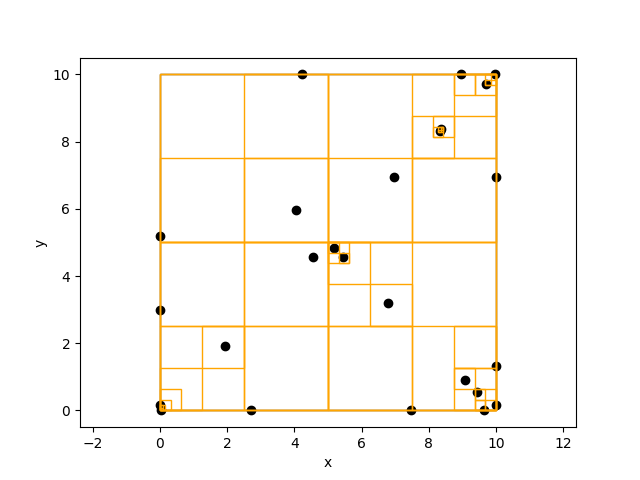
\includegraphics[width=7.9cm]{obrazy/png/rectangle_with_diagonals_test_quad.png} }}%
    \qquad
    \subfloat[\centering Prostokąt i przekątne - KdTree]{{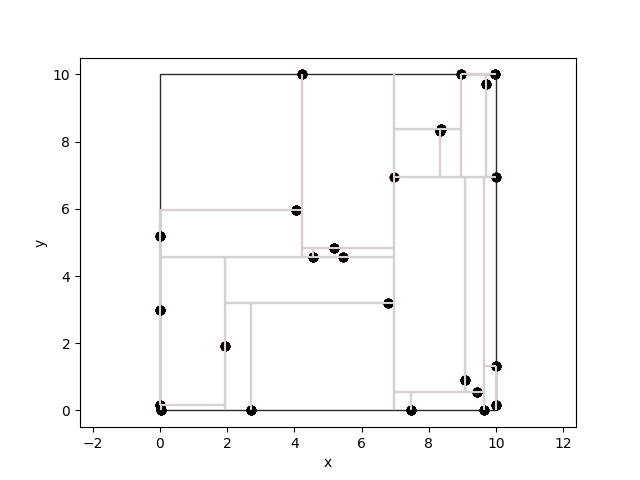
\includegraphics[width=7.9cm]{obrazy/png/rectangle_with_diagonals_test_kd.png} }}%
    \caption{Struktury po inicjalizacji dla testu "Prostokąt i przekątne"}%
    \label{fig:rectangle_with_diagonals}%
\end{figure}

\begin{figure}[h]
    \centering
    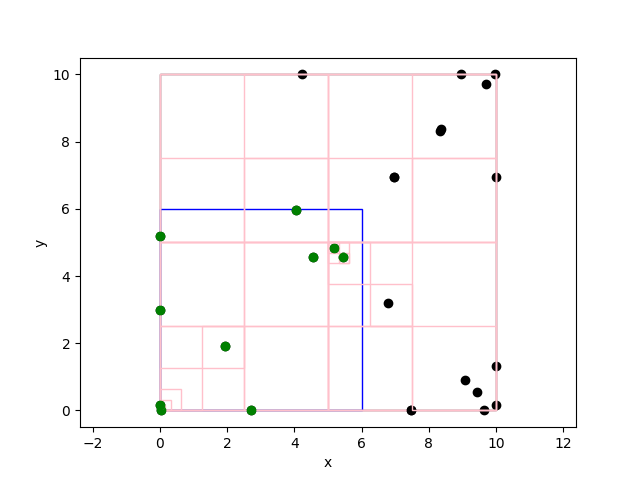
\includegraphics[width=0.6\linewidth]{obrazy/png/rectangle_with_diagonals_test_quad_result.png}
    \caption{Wykres przedstawiający wynik testu "Prostokąt i przekątne" dla \texttt{QuadTree}
    \\
    } 
    W przypadku tej wizualizacji w celu lepszego zobrazowania geometrii przypadku testowego zmieniono wartość parametru \( n = 25 \) na \( n = 100 \) 
    
    \label{fig:rectangle_with_diagonals_test_quad_result}
\end{figure}

\begin{table}[h]
\centering
\caption{Wyniki dla testu "Prostokąt i przekątne"}
\label{tab:rectangle_with_diagonals}
\begin{tabular}{ccccc}
\toprule
\multirow{2}{*}{\textbf{Rozmiar}} & \multicolumn{2}{c}{\textbf{Czas budowy [s]}} & \multicolumn{2}{c}{\textbf{Czas zapytania [s]}} \\
\cmidrule(lr){2-3} \cmidrule(lr){4-5}
 & \textbf{KD} & \textbf{Quad} & \textbf{KD} & \textbf{Quad} \\
\midrule
1000   & 0.019153 & 0.060080 & 0.000320 & 0.000430 \\
5000   & 0.093638 & 0.289424 & 0.001425 & 0.002122 \\
10000  & 0.172475 & 0.607324 & 0.002834 & 0.004014 \\
20000  & 0.367123 & 1.205922 & 0.005619 & 0.008280 \\
40000  & 0.746430 & 2.427409 & 0.011536 & 0.017423 \\
60000  & 1.101405 & 3.672487 & 0.017040 & 0.026337 \\
80000  & 1.460210 & 5.005878 & 0.023141 & 0.037441 \\
100000 & 1.817399 & 6.209093 & 0.029398 & 0.048064 \\
\bottomrule
\end{tabular}
\end{table}


\begin{figure}[h]
    \centering
    \includegraphics[width=1\linewidth]{obrazy/tests/rectangle_with_diagonals_test.png}
    \caption{Wykres porównujący wydajność QuadTree i KdTree dla testu "Prostokąt i przekątne"}
    \label{fig:rectangle_with_diagonals_tests}
\end{figure}
\newpage
\noindent Z analizy tabeli (\ref{tab:rectangle_with_diagonals}) oraz wykresu (\ref{fig:rectangle_with_diagonals_tests}) wynika, że \texttt{KdTree} przewyższa \texttt{QuadTree} pod względem czasu budowy i zapytań w przypadku danych rozmieszczonych na bokach i przekątnych prostokąta. Czas budowy \texttt{KdTree} jest krótszy o około 70\%, co wynika z bardziej efektywnego zarządzania podziałem przestrzeni w tej strukturze.

\noindent Czas zapytań \texttt{KdTree} również jest zauważalnie krótszy (około 40\%), co oznacza, że struktura ta lepiej radzi sobie z obsługą danych o bardziej złożonej geometrii. Na wykresach w skali logarytmicznej widać wyraźną przewagę \texttt{KdTree} dla wszystkich analizowanych rozmiarów danych.

\newpage
\subsection{Dwie chmury}
Dane zgrupowane w dwóch oddzielnych skupiskach pozwalają na ocenę efektywności struktur w sytuacjach, gdy dane są naturalnie pogrupowane.
\begin{itemize}
    \item \textbf{Opis}: Punkty rozmieszczone w dwóch oddalonych od siebie skupiskach w przestrzeni dwuwymiarowej.
    \item \textbf{Prostokąt przeszukiwania}: Centralna część przestrzeni między skupiskami.
    \item \textbf{Zastosowanie}: Analiza wydajności struktur dla danych z grupowaniem.
\end{itemize}



\begin{figure}[h]
    \centering
    \subfloat[\centering Dwie chmury - QuadTree]{{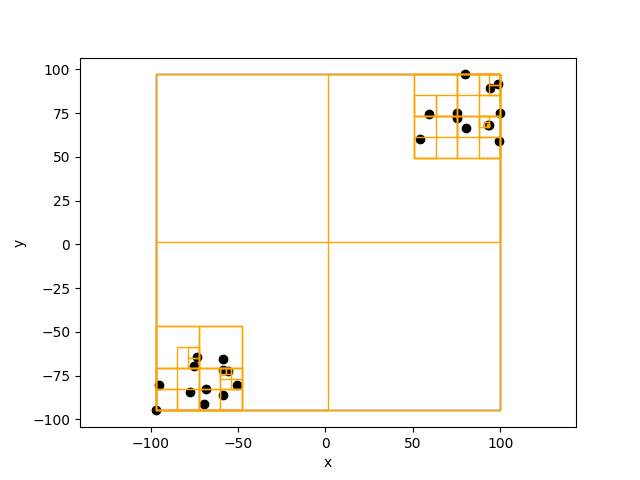
\includegraphics[width=7.9cm]{obrazy/png/test_two_clusters_quad.png} }}%
    \qquad
    \subfloat[\centering Dwie chmury - KdTree]{{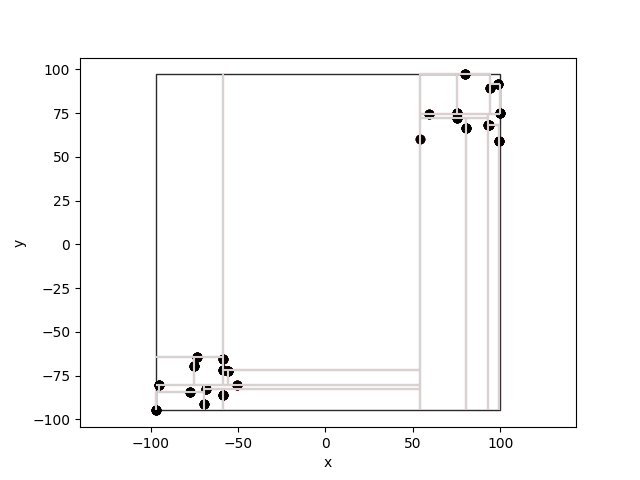
\includegraphics[width=7.9cm]{obrazy/png/test_two_clusters_kd.png} }}%
    \caption{Struktury po inicjalizacji dla testu "Dwie chmury"}%
    \label{fig:two_clusters}%
\end{figure}

\begin{figure}[h]
    \centering
    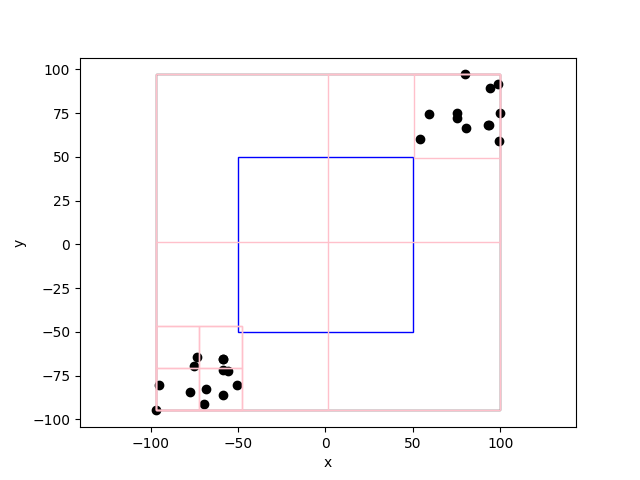
\includegraphics[width=0.6\linewidth]{obrazy/png/test_two_clusters_quad_result.png}
    \caption{Wykres przedstawiający wynik testu "Dwie chmury" dla \texttt{QuadTree}}
    \label{fig:two_clusters_test_quad_result}
\end{figure}

\begin{table}[h]
\centering
\caption{Wyniki dla testu "Dwie chmury"}
\label{tab:test_two_clusters}
\begin{tabular}{ccccc}  % All columns centered
\toprule
\multirow{2}{*}{\textbf{Rozmiar}} & \multicolumn{2}{c}{\textbf{Czas budowy [s]}} & \multicolumn{2}{c}{\textbf{Czas zapytania [s]}} \\
\cmidrule(lr){2-3} \cmidrule(lr){4-5}
 & \textbf{KD} & \textbf{Quad} & \textbf{KD} & \textbf{Quad} \\
\midrule
1000   & 0.018864 & 0.061030 & 0.000187 & 0.000258 \\
5000   & 0.093436 & 0.255466 & 0.000707 & 0.001145 \\
10000  & 0.170613 & 0.566749 & 0.001398 & 0.001942 \\
20000  & 0.365370 & 1.060153 & 0.002911 & 0.004075 \\
40000  & 0.736443 & 2.198701 & 0.005730 & 0.008179 \\
60000  & 1.083175 & 3.303285 & 0.008441 & 0.012393 \\
80000  & 1.437556 & 4.266818 & 0.010866 & 0.015856 \\
100000 & 1.795676 & 5.363671 & 0.013838 & 0.020351 \\
\bottomrule
\end{tabular}
\end{table}

\begin{figure}[h]
    \centering
    \includegraphics[width=1\linewidth]{obrazy/tests/test_two_clusters.png}
    \caption{Wykres porównujący wydajność QuadTree i KdTree dla testu "Dwie chmury"}
    \label{fig:two_clusters_tests}
\end{figure}
\newpage
\noindent Wyniki w tabeli (\ref{tab:test_two_clusters}) oraz wykresu (\ref{fig:two_clusters_tests}) wskazują, że \texttt{KdTree} lepiej radzi sobie z danymi zgrupowanymi w dwóch oddalonych klastrach pod względem czasu budowy. Struktura ta wykazuje krótszy czas budowy, średnio o około 55\%, co wynika z efektywnego zarządzania przestrzenią w podziale hierarchicznym.

\noindent W przypadku czasu zapytań, \texttt{QuadTree} nieznacznie przewyższa \texttt{KdTree}, co jest szczególnie widoczne przy większych zbiorach danych. Ta różnica może wynikać z precyzyjnego podziału przestrzeni na mniejsze podobszary w \texttt{QuadTree}, co ułatwia szybkie lokalizowanie klastrów danych i odrzucenie nieprzecinających się obszarów danych. Na wykresie w skali logarytmicznej widać, że różnice w czasie zapytań między strukturami są minimalne, jednak \texttt{QuadTree} wykazuje niewielką przewagę.


\newpage
\subsection{Punkty odstające}
Dodanie punktów odstających umożliwia analizę odporności struktur na dane niejednorodne, co jest kluczowe w zastosowaniach rzeczywistych, gdzie dane często zawierają anomalie.
\begin{itemize}
    \item \textbf{Opis}: Punkty generowane równomiernie w przestrzeni dwuwymiarowej, z dodatkowymi punktami odstającymi.
    \item \textbf{Prostokąt przeszukiwania}: Fragment przestrzeni centralnej.
    \item \textbf{Zastosowanie}: Ocena odporności struktur na dane odstające.
\end{itemize}

\begin{figure}[h]
    \centering
    \subfloat[\centering Punkty odstające - QuadTree]{{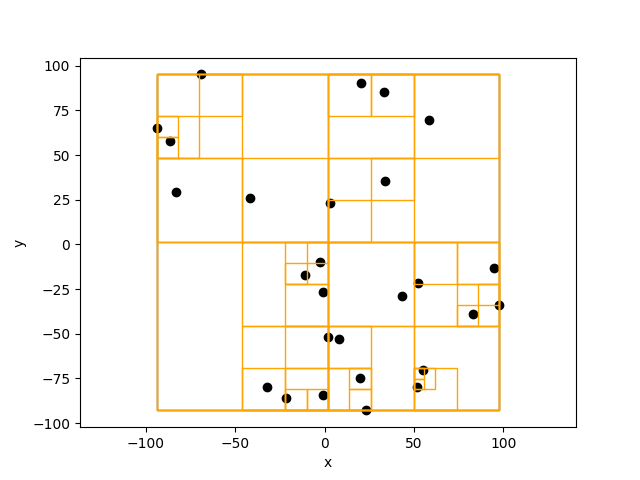
\includegraphics[width=7.9cm]{obrazy/png/test_with_outliers_quad.png} }}%
    \qquad
    \subfloat[\centering Punkty odstające - KdTree]{{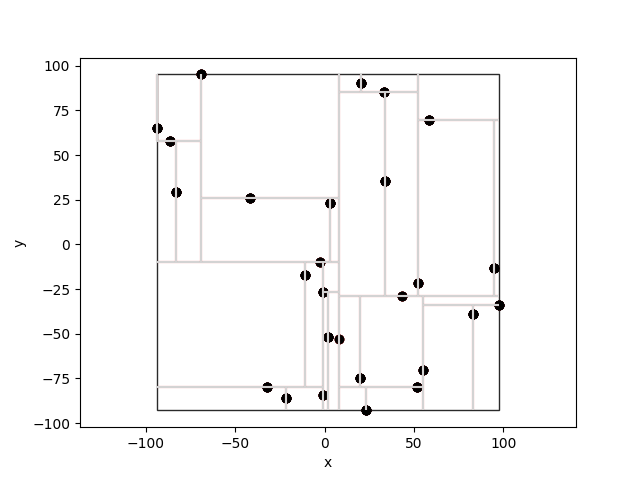
\includegraphics[width=7.9cm]{obrazy/png/test_with_outliers_kd.png} }}%
    \caption{Struktury po inicjalizacji dla testu "Punkty odstające"}%
    \label{fig:outliers}%
\end{figure}

\begin{figure}[h]
    \centering
    \includegraphics[width=0.6\linewidth]{obrazy/png/test_with_outliers_quad_result.png}
    \caption{Wykres przedstawiający wynik testu "Punkty odstające" dla \texttt{QuadTree}}
    \label{fig:test_with_outliers_quad_result}
\end{figure}

\begin{table}[h]
\centering
\caption{Wyniki dla testu "Punkty odstające"}
\label{tab:test_with_outliers}
\begin{tabular}{ccccc}
\toprule
\multirow{2}{*}{\textbf{Rozmiar}} & \multicolumn{2}{c}{\textbf{Czas budowy [s]}} & \multicolumn{2}{c}{\textbf{Czas zapytania [s]}} \\
\cmidrule(lr){2-3} \cmidrule(lr){4-5}
 & \textbf{KD} & \textbf{Quad} & \textbf{KD} & \textbf{Quad} \\
\midrule
1000   & 0.021582 & 0.062748 & 0.000558 & 0.000762 \\
5000   & 0.100999 & 0.300314 & 0.002600 & 0.004104 \\
10000  & 0.204854 & 0.590257 & 0.005725 & 0.007443 \\
20000  & 0.400047 & 1.226448 & 0.010727 & 0.015833 \\
40000  & 0.798416 & 2.312280 & 0.021072 & 0.032199 \\
60000  & 1.177021 & 3.569608 & 0.032670 & 0.049806 \\
80000  & 1.566542 & 4.958558 & 0.046899 & 0.071353 \\
100000 & 1.947802 & 6.247821 & 0.054815 & 0.085537 \\
\bottomrule
\end{tabular}
\end{table}
\begin{figure}[h]
    \centering
    \includegraphics[width=1\linewidth]{obrazy/tests/test_with_outliers.png}
    \caption{Wykres porównujący wydajność QuadTree i KdTree dla testu "Punkty odstające"}
    \label{fig:test_with_outliers}
\end{figure}
\newpage
\noindent Wyniki w tabeli (\ref{tab:test_with_outliers}) oraz wykresu (\ref{fig:test_with_outliers}) pokazują, że w przypadku danych z punktami odstającymi, \texttt{KdTree} wykazuje lepsze wyniki zarówno w czasie budowy, jak i w czasie zapytań. Czas budowy \texttt{KdTree} jest krótszy o około 65\%, co świadczy o efektywności tej struktury w generowaniu hierarchii nawet w obecności danych odstających.

\noindent W przypadku czasu zapytań, \texttt{KdTree} również utrzymuje przewagę nad \texttt{QuadTree}, co można przypisać wydajnemu podziałowi przestrzeni i redukcji liczby sprawdzanych węzłów.

\newpage
\section{Podsumowanie wyników testów wydajnościowych}
Na podstawie wyników testów przedstawionych w tabelach i wykresach można zauważyć istotne różnice w wydajności struktur \texttt{QuadTree} i \texttt{KdTree}, w zależności od charakterystyki danych.

\subsection{Zbiorcza analiza czasu budowy}

\noindent \textbf{\texttt{KdTree} przewyższa \texttt{QuadTree} w czasie budowy} w większości przypadków testowych, co jest szczególnie widoczne dla dużych zbiorów danych oraz scenariuszy z równomiernym lub nieregularnym rozmieszczeniem punktów. 

\begin{itemize}
    \item \textbf{Największa przewaga \texttt{KdTree}:}
    \begin{itemize}
        \item \texttt{Rozkład jednostajny}: Czas budowy krótszy o około 60–65\%.
        \item \texttt{Prostokąt i przekątne}: Redukcja czasu budowy o około 70\%.
        \item \texttt{Punkty odstające}: Czas budowy krótszy o 65\%.
    \end{itemize}
    
    \item \textbf{Scenariusze o porównywalnych wynikach:}
    \begin{itemize}
        \item W testach takich jak \texttt{Boki prostokąta} oraz \texttt{Prosta}, \texttt{QuadTree} w niektórych przypadkach przewyższa \texttt{KdTree}, szczególnie przy danych geometrycznie dostosowanych do podziałów stosowanych w \texttt{QuadTree}. Dla danych o regularnym rozmieszczeniu na bokach prostokąta, \texttt{QuadTree} wykazała krótszy czas budowy przy większych zbiorach danych.
    \end{itemize}
\end{itemize}

\subsection{Zbiorcza analiza czasu zapytań}

\noindent \textbf{W przypadku czasu zapytań różnice między strukturami były bardziej zróżnicowane i zależały od charakterystyki danych.}

\begin{itemize}
    \item \textbf{Scenariusze z przewagą \texttt{QuadTree}:}
    \begin{itemize}
        \item \texttt{Okrąg}: Dzięki mechanizmowi precyzyjnego odrzucania obszarów nieprzecinających się, \texttt{QuadTree} osiągnęła minimalnie lepszy czas zapytań.
        \item \texttt{Dwie chmury}: \texttt{QuadTree} była nieco szybsza w zapytaniach, co wynika z lepszego podziału przestrzeni na mniejsze fragmenty przy danych klastrowych.
    \end{itemize}
    
    \item \textbf{Scenariusze z przewagą \texttt{KdTree}:}
    \begin{itemize}
        \item \texttt{Prostokąt i przekątne} oraz \texttt{Punkty odstające}: \texttt{KdTree} utrzymała przewagę w zapytaniach, co wynika z efektywności hierarchicznego podziału przestrzeni.
        \item Testy \texttt{Prosta} i \texttt{Krzyż}: W przypadku danych liniowych lub osiowych, czas zapytań w \texttt{KdTree} był krótszy o około 35–40\%.
    \end{itemize}
\end{itemize}

\subsection{Podsumowanie:}


\noindent Obie struktury wykazały wysoką efektywność w odpowiednich zastosowaniach, jednak wybór jednej z nich powinien być dostosowany do charakterystyki danych.

\newpage
\section{Testy \texttt{QuadTree} dla różnych wartości \texttt{max\_capacity}}

Przeprowadzono testy dla różnych wartości \texttt{max\_capacity}, aby sprawdzić ich wpływ na czas budowy i czas zapytań drzewa QuadTree. Testy wykonano na losowym zbiorze danych (Test: Rozkład Jednostajny) o rozmiarze \( n = 5000 \). Parametr \texttt{max\_capacity} zmieniał się w zakresie \( 1 \)–\( 100 \):
\( 1 \)–\( 20 \) (z krokiem \( 1 \)) oraz \( 20 \)–\( 100 \) (z krokiem \( 5 \)).

\subsection{Czas budowy QuadTree}
\begin{itemize}
    \item Czas budowy maleje wraz ze wzrostem wartości \texttt{max\_capacity}, co widać na rysunku (\ref{fig:max_cap}a) z naniesioną linią regresji.
    \item Przy niskich wartościach \texttt{max\_capacity} (np. \( 1 \)–\( 20 \)) czas budowy jest dłuższy z powodu konieczności budowy głębszego drzewa z większą liczbą węzłów.
    \item Dla wyższych wartości \texttt{max\_capacity} (np. \( 20 \)–\( 100 \)), czas budowy stabilizuje się, ponieważ drzewo staje się płytsze, a liczba operacji podziału maleje.
\end{itemize}

% \begin{figure}[h]
%     \centering
%     \includegraphics[width=0.5\textwidth]{obrazy/line_bud.png}
%     \caption{Wykres czasu budowy QuadTree w zależności od \texttt{max\_capacity} z linią regresji.}
%     \label{fig:line_bud}
% \end{figure}

\subsection{Czas zapytań w QuadTree}
\begin{itemize}
    \item Czas zapytań rośnie wraz ze wzrostem wartości \texttt{max\_capacity}, co widać na rysunku (\ref{fig:max_cap}b) z naniesioną linią regresji
    \item Dla niskich wartości \texttt{max\_capacity} zapytania są bardziej efektywne, ponieważ głębsze drzewo umożliwia szybkie dotarcie do odpowiednich węzłów.
    \item Dla wysokich wartości \texttt{max\_capacity}, zapytania są mniej efektywne, ponieważ płytsze drzewo wymaga przeszukania większej liczby punktów w jednym węźle.
\end{itemize}


\begin{figure}[h]
    \centering
    \subfloat[\centering Czas Budowy]{{\includegraphics[width=7.9cm]{obrazy/line_bud.png} }}%
    \qquad
    \subfloat[\centering Czas Zapytań]{{\includegraphics[width=7.9cm]{obrazy/line_zap.png} }}%
    \caption{Wykres czasu zapytań QuadTree w zależności od \texttt{max\_capacity} z linią regresji.}%
    \label{fig:max_cap}%
\end{figure}


\subsection{Podsumowanie}

Wyniki testów potwierdzają teoretyczne zależności dla struktury \texttt{QuadTree}. Parametr \texttt{max\_capacity} ma kluczowy wpływ na wydajność drzewa w zależności od zastosowań.
Dla zbudowania jednej struktury i obsługi wielu zapytań, ustawienie domyślnej wartości \texttt{max\_capacity = 4} wydaje się być optymalnym kompromisem pomiędzy czasem budowy a czasem zapytań, zwłaszcza w przypadku, gdy dla ustalonego zbioru punktów chcemy wielokrotnie przeszukiwać różne ustalone obszary.
\newpage

\section{Wnioski i Podsumowanie}

Na podstawie przeprowadzonych testów i analizy działania zaimplementowanych struktur danych, można stwierdzić, że zarówno \texttt{QuadTree}, jak i \texttt{KdTree} działają poprawnie, skutecznie wyznaczając podzbiory punktów należących do zadanej płaszczyzny. Obydwie struktury wykazały swoje mocne strony w zależności od charakterystyki zbiorów danych i scenariuszy zastosowania.

\subsection{Wnioski}
\begin{itemize}
    \item \textbf{Czas konstrukcji:} 
    \begin{itemize}
        \item W większości przypadków \texttt{KdTree} osiąga krótsze czasy budowy, szczególnie dla dużych i równomiernych zbiorów danych. Struktura ta skutecznie zarządza hierarchicznym podziałem przestrzeni, co przekłada się na wyższą wydajność w tym aspekcie.
        \item \texttt{QuadTree} wykazuje konkurencyjność w budowie przy zbiorach, które mają naturalną geometrię dostosowaną do jej sposobu podziału przestrzeni, takich jak dane współliniowe czy dane na krawędziach.
    \end{itemize}
    
    \item \textbf{Czas zapytań:}
    \begin{itemize}
        \item \texttt{KdTree} osiąga lepsze wyniki dla gęsto usianych danych o regularnych rozkładach, takich jak rozkład normalny czy jednolity. Dzięki swojej strukturze odwiedza mniej węzłów podczas przeszukiwania.
        \item \texttt{QuadTree} wykazuje przewagę dla rzadkich zbiorów danych, współliniowych rozmieszczeń oraz bardziej nieregularnych geometrii. Jej sposób podziału przestrzeni pozwala szybko odcinać nieistotne węzły, co skutkuje krótszymi czasami zapytań.
    \end{itemize}
    
    \item \textbf{Ogólna wydajność:}
    \begin{itemize}
        \item \texttt{KdTree} jest lepszym wyborem w sytuacjach, gdy mamy do czynienia z dużymi zbiorami danych i ich rozkład jest nieznany. Jego wszechstronność sprawia, że nadaje się do wielu scenariuszy aplikacyjnych.
        \item \texttt{QuadTree} jest bardziej efektywna w przypadku specyficznych rozkładów danych, szczególnie gdy dane są zlokalizowane na krawędziach przestrzeni lub mają charakterystyczną, rzadką geometrię.
    \end{itemize}
\end{itemize}

\subsection{Podsumowanie}

Podsumowując, wybór odpowiedniej struktury danych powinien być uzależniony od charakterystyki zbioru danych i celu analizy. W ogólnych przypadkach \texttt{KdTree} jest bardziej uniwersalne, natomiast \texttt{QuadTree} sprawdza się w szczególnych scenariuszach, gdzie nieregularna geometria danych odgrywa kluczową rolę.

\newpage
\pagestyle{plain}
\section*{Bibliografia}
\noindent Źródła i inspiracje wykorzystane przy tworzeniu projektu:
\begin{itemize}
  \item Wykłady z Algorytmów Geometrycznych, prowadzone przez dr inż. Barbarę Głut
  \item \url{https://github.com/aghbit/Algorytmy-Geometryczne} -- Narzędzie do wizualizacji
  \item \url{https://en.wikipedia.org/wiki/Quadtree}
  \item \url{https://en.wikipedia.org/wiki/K-d_tree}
  \item \url{https://www.agh.edu.pl/o-agh/multimedia/znak-graficzny-agh/}
  \item \url{https://github.com/Goader/KDTree_QuadTree/tree/main} -- Wybrane przypadki testowe
  \item \url{https://home.agh.edu.pl/~polak/pl.php} -- Motyw Beamer
\end{itemize}
\section*{Autorzy implementacji}
Implementacja poszczególnych struktur danych:
\begin{itemize}
  \item QuadTree - Maciej Kmąk
  \item KdTree - Michał Szymocha
\end{itemize}

\end{document}
